\documentclass[aspectratio=169]{beamer}
\usepackage[utf8]{inputenc}

\setbeamersize{text margin left=3mm,text margin right=3mm} 

\usetheme{Oxygen}
\usepackage{hyperref}
%\usepackage{movie15}
\usepackage{textpos}
\usepackage{fancybox}
\usepackage{colortbl}
\usepackage{rotating}
\usepackage{pgfplots}
\pgfplotsset{compat=1.18}
\usepackage{ragged2e}
% \usepackage{subfigure}
%\usepackage{subcaption}
\usepackage{multicol}
\usepackage{multirow}
\usepackage{amsmath,amssymb,amsfonts,amsbsy,dsfont}
\usepackage{mathrsfs}
\usepackage{amsthm}
\usepackage{bm}
\usepackage{array}
%\usepackage[caption=false]{subfig}
\usepackage{arydshln}
\usepackage{breakcites}
\usepackage{booktabs}
\usepackage{tabularx}
\usepackage{makecell}
\usepackage{amsmath}
\usepackage{tikz}
\usepackage{pgf-pie}
\usepackage{epsfig,epic,eepic,threeparttable,amscd,here,lscape,tabularx,graphicx }
\usepackage{booktabs}
\usepackage{tabu,array}
\usepackage{overpic}
\usepackage{microtype}

\usepackage{subcaption}
\usetikzlibrary{decorations.pathreplacing}

\definecolor{GII}{RGB}{255,255,107}
\definecolor{GI}{RGB}{72,197,72}
\definecolor{GIII}{RGB}{214, 36, 47}

\colorlet{color0}{blue!40!gray}% pearson *
\colorlet{color1}{blue!80!gray} %pearson **
\colorlet{color2}{red!40!gray} %n-pearson*
\colorlet{color3}{red!80!gray}%n-pearson**
\colorlet{color4}{green!40!gray} %plv*
\colorlet{color5}{green!80!gray} 


\definecolor{GI_b}{RGB}{255, 233, 0}
\definecolor{GII_b}{RGB}{0, 140, 140}
\definecolor{GIII_b}{RGB}{74, 0, 74}
% yellow
% purple
% turquoise

\newcommand{\lineplot}[1]{
	\tikz[baseline=-0.5ex] \draw[#1,thick] (0,0) -- (0.3,0);
}

\newcommand{\dashlineplot}[1]{
    \tikz[baseline=-0.5ex] \draw[#1, dashed, thick] (0,0) -- (0.3,0);
}

% \providecommand{\ppunto}[2]{\langle#1, #2 \rangle}% producto punto
% \providecommand{\promed}[1]{{\mathbb{E}}\left\lbrace #1\right\rbrace}% operador de promedio
% \providecommand{\promeddd}[2]{\mathbb{E}_{#1}\!\left\{#2\right\}}% op{\tiny }erador de promedio
% \providecommand{\promedd}[2]{\mathds{E}_{#1}\left\{#2\right\}}% operador de promedio
% \providecommand{\cov}[2]{{\fam=7 cov}\{#1, #2\}}% operador de covarianza
% \providecommand{\gaus}[2]{{\fam=6 N}(#1 #2)} % FDP Gauss
% % Kronecker delta function
% \providecommand{\Kronecker}[2]{\delta_{K}( #1 , #2 )}
% % cardinality
% \providecommand{\Cardinality}[1]{| #1 |}

\let\oldcite\cite % store the original \cite command
\renewcommand{\cite}[1]{{\tiny\oldcite{#1}}}

\usepackage{bm}

\usepackage{etoolbox}

\DeclareUnicodeCharacter{2212}{-}

\DeclareRobustCommand{\legend}[1]{%
	\textcolor{#1}{\rule{1ex}{2ex}}%
}

\newcommand{\ve}[1]{\bm {#1}}
\newcommand{\mat}[1]{\bm {#1}}
\usepackage[nopar]{lipsum} 

\newif\ifcomment
\newcommand{\Com}{\par\footnotesize\itshape\commenttrue}

\newenvironment{Itemize}
 {%
  \edef\Itemizecurrent{\the\font}%
  \itemize
  \preto{\item}{\ifcomment\par\Itemizecurrent\fi}%
 }{%
  \enditemize
 }


\title[An Embedded Deep Learning Approach for
Seed Image Segmentation - Camilo Pelaez Garcia]{An Embedded Deep Learning Approach for
Seed Image Segmentation}
\vskip -0.7cm
\author{\normalsize{Camilo Pelaez Garcia}\\ \scriptsize{cpelaezg@unal.edu.co
}}
\institute{
\includegraphics[width=0.15\textwidth]{EscudoUN-2016.png}\\\scriptsize{
Universidad Nacional de Colombia - Sede Manizales \\ Signal Processing and Recognition Group - SPRG
\\
\textbf{Advisor:} Andrés Marino Álvarez-Meza, Ph.D.\\
\vspace{-0.3cm}
}}

% \date[]{Department of Electrical, Electronic and Computer Engineering\\
% Universidad Nacional de Colombia - Sede Manizales}
\date[]{\scriptsize{2025}}



\setbeamercovered{dynamic}
\setbeamertemplate{navigation symbols}{}
\begin{document}

{\setbeamertemplate{headline}{}
\setbeamertemplate{footline}{}
\begin{frame}{}
    \vspace{-0.7cm}
        \titlepage 
\end{frame}
}


\newif\iflattersubsect

\AtBeginSection[] {
    \begin{frame}
    \frametitle{Outline} %
    \tableofcontents[currentsection, sections={1-6}]  
    \end{frame}
    \lattersubsectfalse
}

\AtBeginSection[] {
    \begin{frame}
    \frametitle{Outline I} %
    \tableofcontents[currentsection, sections={1-6}]  
    \end{frame}
    \only<7-9>{
        \begin{frame}
        \frametitle{Outline II} %
        \tableofcontents[currentsection, sections={7-9}]  
        \end{frame}
    }
    \lattersubsectfalse
}

\AtBeginSection[] {
    \ifnum\thesection<7
        \begin{frame}
        \frametitle{Outline I} %
        \tableofcontents[currentsection, sections={1-6}]  
        \end{frame}
    \else
        \begin{frame}
        \frametitle{Outline II} %
        \tableofcontents[currentsection, sections={7-11}]  
        \end{frame}
    \fi
    \lattersubsectfalse
}

\AtBeginSubsection[] {
    \ifnum\thesection<7
        \begin{frame}
        \frametitle{Outline I} %
        \tableofcontents[currentsubsection, sections={1-6}]  
        \end{frame}
    \else
        \begin{frame}
        \frametitle{Outline II} %
        \tableofcontents[currentsubsection, sections={7-11}]  
        \end{frame}
    \fi
    \lattersubsectfalse
}

\section[Motivation]{Motivation}

\begin{frame}{Global food security context}
    \begin{columns}
        \column{0.45\textwidth}
            \begin{figure}
                \centering
                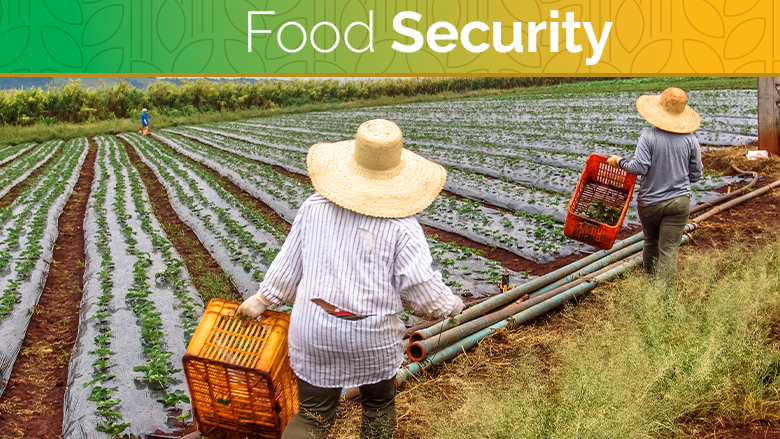
\includegraphics[width=0.95\linewidth]
                {Tesis_presentation/Figures/blog-food-security2.png}
                \caption{\footnotesize \textbf{Image:} Acquired from \href{https://www.weforum.org/}{World Economic Forum 2024}}
            \end{figure}

        \column{0.55\textwidth}
            \begin{itemize}
                \item \textbf{Global Urgency:}
                \textbf{2.3 billion people} faced moderate or severe food insecurity in 2024. Germination is the fundamental first step to secure production~\cite{fao2025sofi}.

                \item \textbf{Yield Bottleneck:}
                Suboptimal germination directly compromises seedling establishment and crop productivity, with minimum acceptable rates of \textbf{85\%} for certified cereal seeds~\cite{finch-savage2016seed, barik2022unraveling}.

                \item \textbf{Controlled Environment:}
                Unlike soil methods, \textbf{in vitro} environments offer the control and standardization required for high-throughput phenotyping~\cite{joosen2020}.
            \end{itemize}
    \end{columns}
\end{frame}

\begin{frame}{Magnetic Seed Treatment (MST) relevance}
    \begin{columns}
        \column{0.4\textwidth}
            \begin{figure}
                \centering
                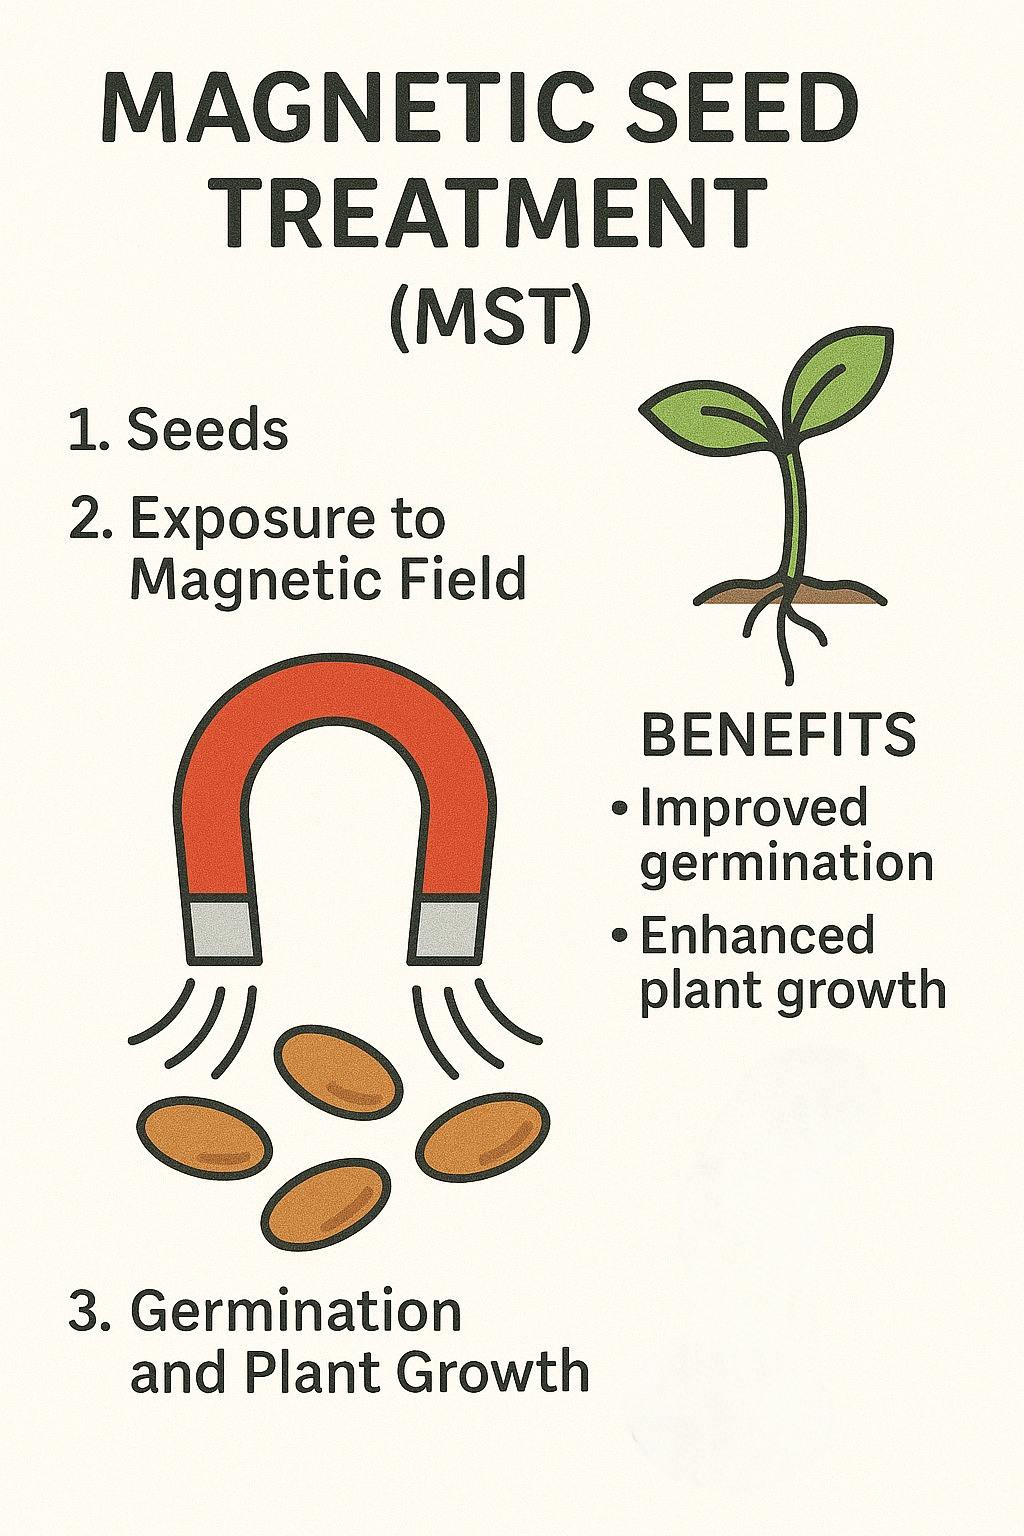
\includegraphics[width=0.75\linewidth]{Tesis_presentation/Figures/seedMTS.jpg}
            \end{figure}

        \column{0.6\textwidth}
            \vspace{-0.5cm}
            \begin{itemize}
                \item \textbf{Germination enhancement:}
                MST increases germination rates by \textbf{20--50\%} and accelerates early growth~\cite{Pietruszewski2015,maffei2014,shah2024directional}.

                \item \textbf{Early morphological changes:}
                Magnetic exposure significantly affects radicle emergence during the first days after sowing~\cite{garcia2019,iqbal2021}.

                \item \textbf{Monitoring challenge:}
                Subtle MST-induced morphological changes make manual evaluation \textbf{slow, subjective and low-throughput}, driving the need for automated, non-invasive monitoring.~\cite{Pietruszewski2015,DeSousa2016Review,maffei2014}.
            \end{itemize}
    \end{columns}
\end{frame}

\begin{frame}{Deep Learning in Seed Germination Monitoring}
    \begin{columns}
        \column{0.45\textwidth}
            \begin{figure}[htbp]
                \centering
                \includegraphics[width=0.85\linewidth, trim={0 100pt 0 100pt}, clip]{Tesis_presentation/Figures/cv_agriculture_tasks.pdf}
                \caption*{\scriptsize Deep Learning tasks in phenotyping \cite{jiang2025image}}
            \end{figure}
        \column{0.55\textwidth}
            \textbf{Core Computer Vision Paradigms:}
            \begin{itemize}
                \setlength\itemsep{0.5em}
                \item \textbf{Classification:}
                Categorizing vigor levels and developmental stages with improved generalizability \cite{kamilaris2018deep}.
                
                \item \textbf{Detection:}
                Localizing seeds for high-throughput counting in dense arrays \cite{liu2022_vision}.
                
                \item \textbf{Segmentation:}
                Pixel-level extraction of morphological traits and temporal dynamics—essential for fine-grained analysis \cite{Minaee2021, luo2024semseg}.
            \end{itemize}
            \vspace{0.3cm}
            \small
            \textit{Enables \textbf{end-to-end} automated phenotyping, replacing subjective manual assessments \cite{linaza2021}.}
    \end{columns}
\end{frame}

\begin{frame}{Semantic Segmentation for Germination Analysis}
    \begin{columns}
        \column{0.35\textwidth}
            \begin{figure}
                \centering                
                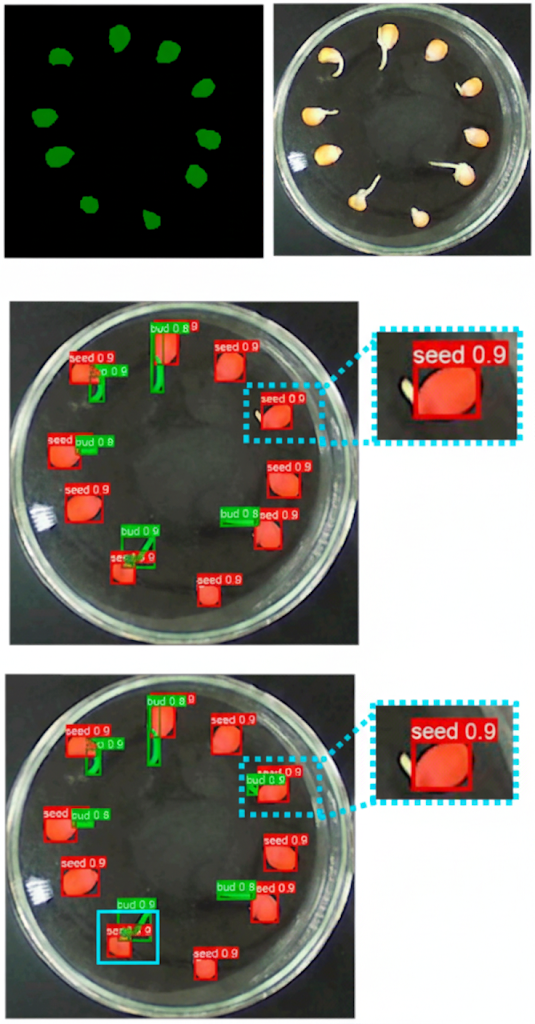
\includegraphics[width=0.6\linewidth]{Tesis_presentation/Figures/segmentation_example_seeds2.png}
                \caption*{\scriptsize Example of seed segmentation \cite{yu2025vt_yolov8_seg}}
            \end{figure}

        \column{0.65\textwidth}
            \textbf{Advantages over standard detection:}
            \begin{itemize}
                \setlength\itemsep{0.6em}
                \item \textbf{Morphological Precision:}
                Accurately measures radicle length, area, and shape, not just bounding boxes \cite{liu2022_vision, zhang2025review}.
                
                \item \textbf{Handling Occlusions:}
                Effective separation of touching seeds or overlapping roots \cite{elmasry2019, liu2022_vision}.
                
                \item \textbf{Early Detection:}
                Captures subtle pixel-level changes (protrusion) invisible to standard inspection \cite{elmasry2019}.
            \end{itemize}
    \end{columns}
\end{frame}

\begin{frame}{Embedded AI Platforms for Agricultural Monitoring}
    \begin{columns}
        \column{0.45\textwidth}
            \begin{figure}[htbp]
                \centering
                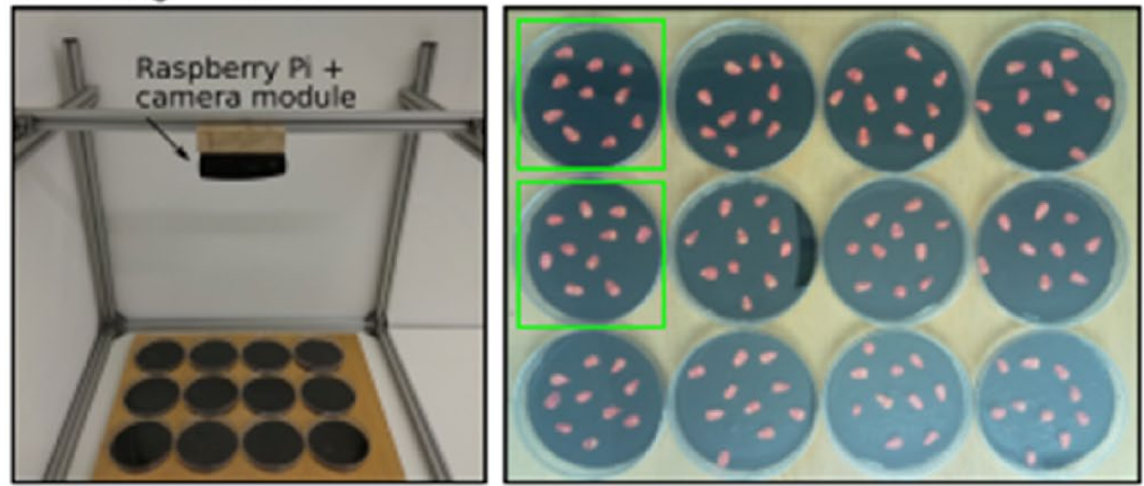
\includegraphics[width=0.8\linewidth]{Tesis_presentation/Figures/embedded_ai_platforms_a.png}
                
                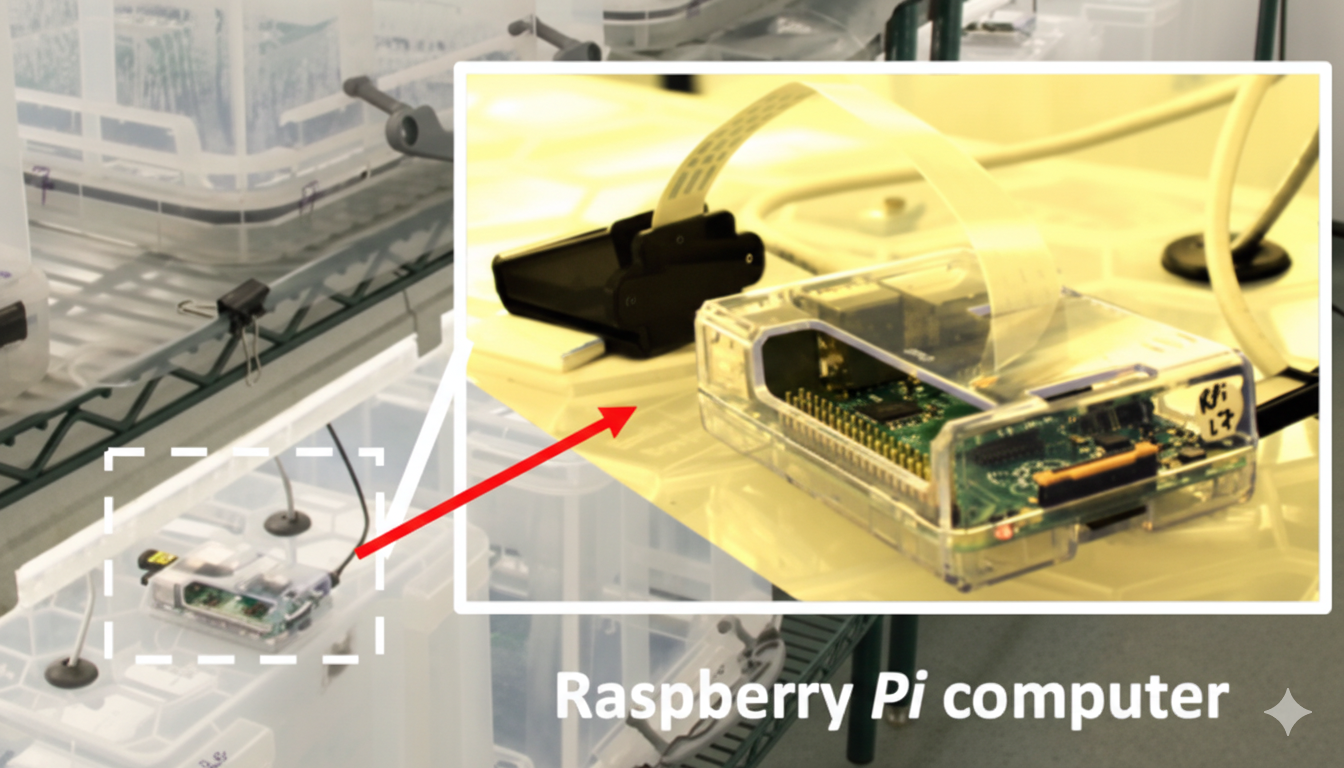
\includegraphics[width=0.8\linewidth]{Tesis_presentation/Figures/embedded_ai_platforms_b.png}
                \caption*{\scriptsize Edge hardware for agricultural monitoring \cite{genze2020accurate, elmasry2019}}
            \end{figure}

        \column{0.55\textwidth}
            \textbf{Enabling Scalable Deployment:}
            \begin{itemize}
                \setlength\itemsep{0.6em}

                \item \textbf{Autonomous Operation:}
                Essential in environments where high-bandwidth connectivity is not guaranteed \cite{rguibi2022deep, gholami2022survey}.
                
                \item \textbf{Raspberry Pi:}
                Standard platforms used due to affordability and ease of integration \cite{genze2020accurate, elmasry2019}.
                
                \item \textbf{Edge Computing Benefits:}
                Reduces latency and avoids prohibitive costs of continuous data streaming \cite{kwon2024hard}.
            \end{itemize}

            \vspace{0.3cm}
            \small
            \textit{Result: Addresses the accuracy, speed, and deployability \textbf{trilemma} \cite{gholami2022survey}.}
    \end{columns}
\end{frame}

\begin{frame}{Local Context: SPRG - UNAL - UdC}
    \begin{columns}
        \column{0.45\textwidth}
            \begin{figure}
                \centering
                \resizebox{0.95\linewidth}{!}{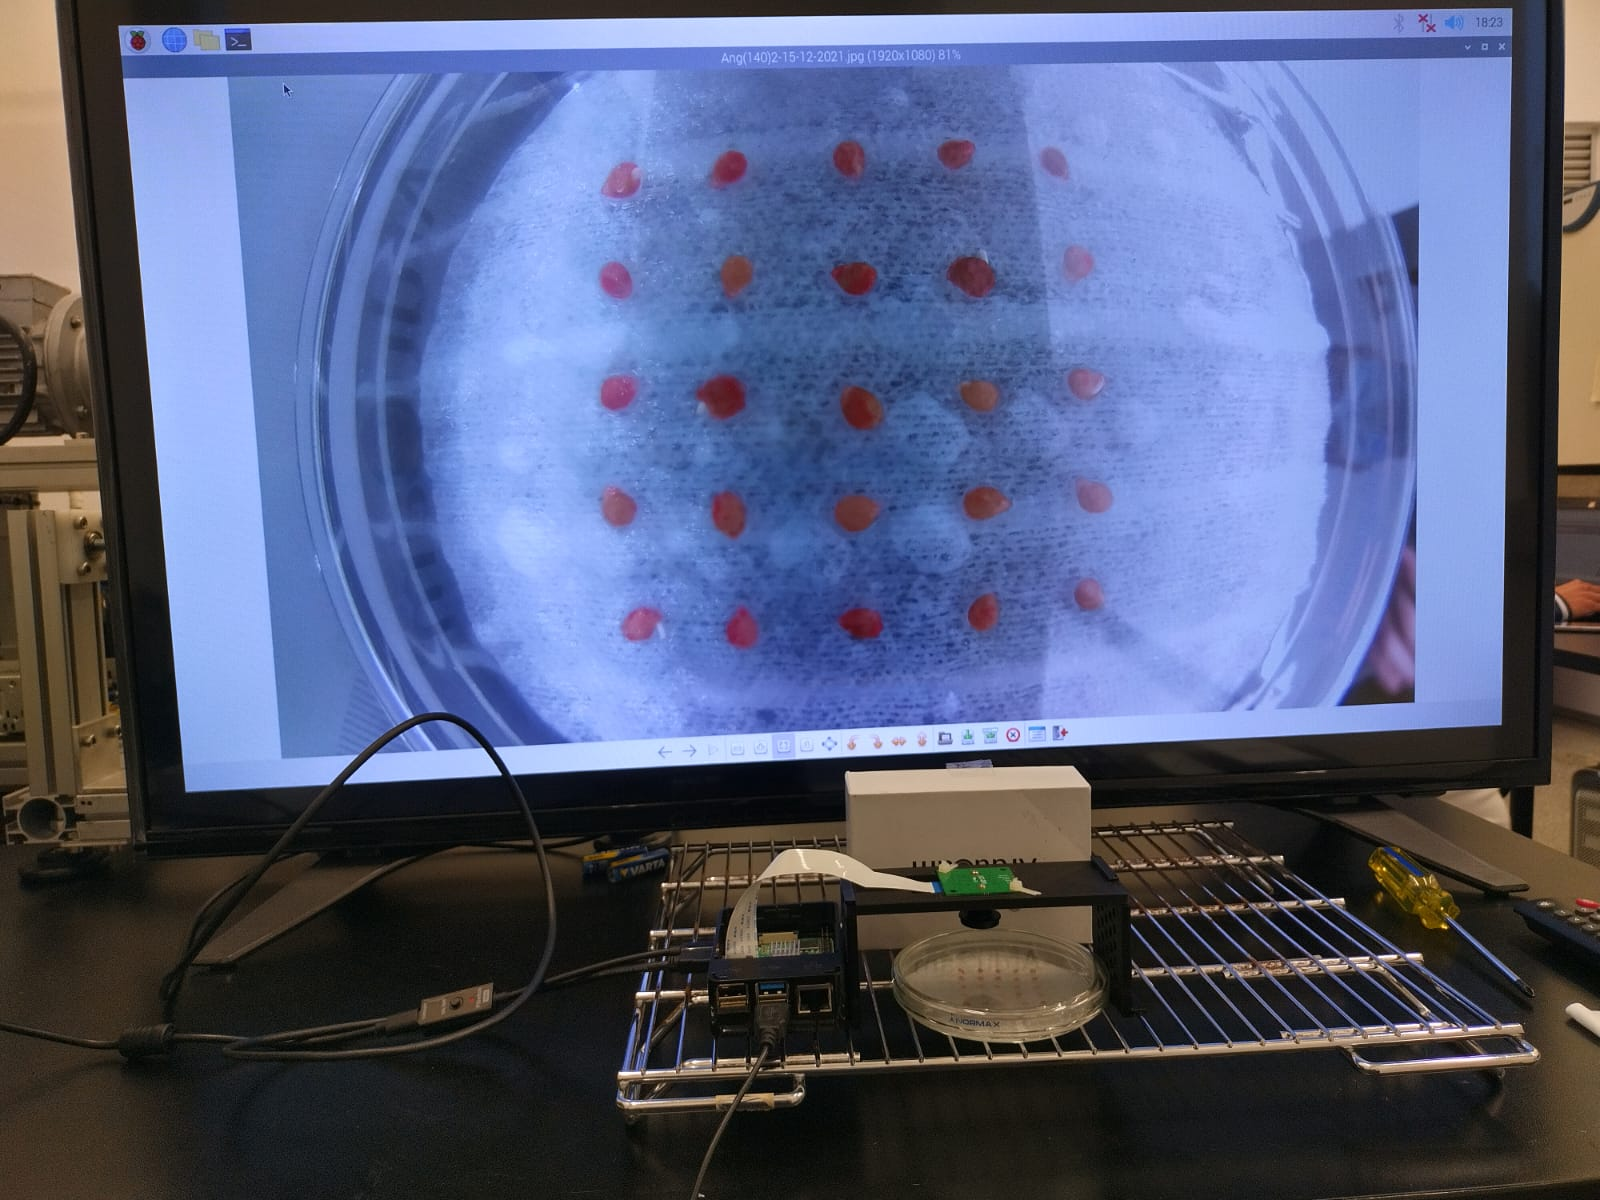
\includegraphics{Tesis_presentation/Figures/prototipo_in_vitro_automation.jpeg}}
            \end{figure}

        \column{0.55\textwidth}
            \small
            \textbf{Applied Computer Vision \& Embedded Deployment:}
            
            \begin{itemize}
                \setlength\itemsep{0.3em} % Reduce espacio entre items
                
                \item \textbf{Food Security (Hermes 54339):}
                CV tool for plant analysis aimed at strengthening food security strategies.
                
                \item \textbf{In Vitro Automation (Hermes 49592):}
                \textit{Precursor project.} Automated prototype for \textit{in vitro} germination analysis using computer vision.
                
                \item \textbf{Maternal Health (Hermes 57661):}
                Monitoring system for anesthetic effects at \textit{SES HUC}, validating deployment on edge devices in critical scenarios.
            \end{itemize}
            
            \vspace{0.5em}
            \footnotesize
            \textbf{Thesis Continuity:} This work extends \textbf{Hermes 49592}, evolving the prototype towards \textbf{Deep Learning} and \textbf{Edge AI}.
    \end{columns}
\end{frame}


\section{Problem statement}

\begin{frame}{Problem Statement}
    \centering
    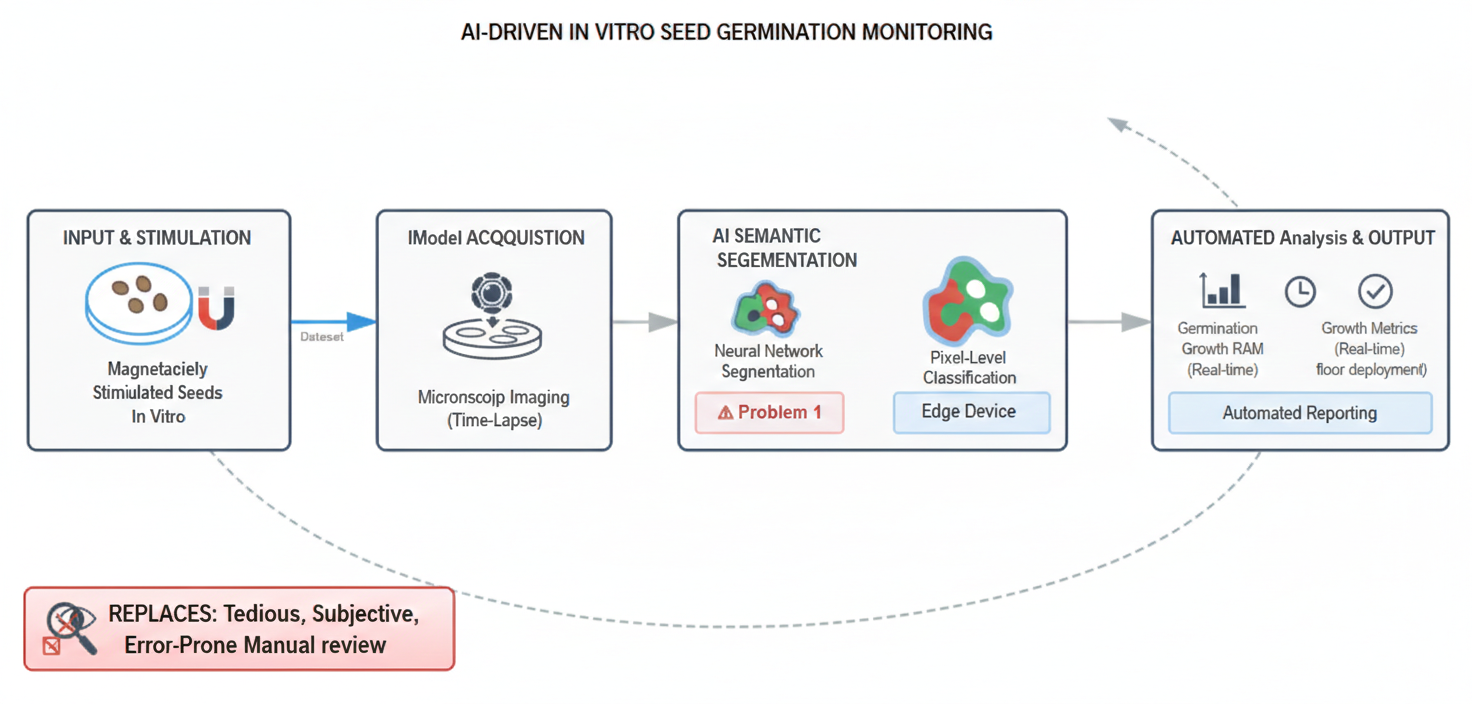
\includegraphics[width=0.7\linewidth]{./Tesis_presentation/Figures/general-problem.pdf}
    \footnotetext[1]{\scriptsize\textcolor{red!70!black}{Manual limitations: \cite{jin2025application, jin2023label, joosen2010germinator}}}
    \footnotetext[2]{\scriptsize\textcolor{green!50!black}{AI challenges: \cite{kumar2024image, gholami2022survey, liu2025low}}}
\end{frame}

\begin{frame}{Scarcity of Annotated Datasets}
    \begin{figure}[!ht]
        \centering
        \includegraphics[width=0.7\linewidth]{./Tesis_presentation/Figures/problem1_vf.pdf} 
    \end{figure}
    \footnotetext[1]{\scriptsize Annotation \& data limitations: \cite{jin2023label, wang2024comprehensive, bewley2013seeds, joosen2010germinator}}
    \footnotetext[2]{\scriptsize Model training challenges: \cite{kumar2024image, chlap2021deepmed, chlap2021augmentation}}
\end{frame}

\begin{frame}{Lack of Generalization and Overfitting in Pattern Recognition}
    \begin{figure}[!ht]
        \centering
        \includegraphics[width=0.7\linewidth]{./Tesis_presentation/Figures/problem2_vf.pdf}
    \end{figure}
    \footnotetext[1]{\scriptsize Generalization failures: \cite{ayana2024multistage, halmosi2024evaluating, chlap2021deepmed, kumar2024image}}
    \footnotetext[2]{\scriptsize Fine-grained morphology challenges: \cite{wang2024improved, barreiro2025enhancing, bewley2013seeds, joosen2010germinator}}
\end{frame}


\begin{frame}{Deployment Constraints}
    \begin{figure}[!ht]
        \centering
        \includegraphics[width=0.68\linewidth]{./Tesis_presentation/Figures/problem3_vf.pdf}
    \end{figure}
    \footnotetext[1]{\scriptsize Model requirements vs. edge hardware: \cite{wang2024improved, kwon2024hard, sandler2018mobilenetv2}}
    \footnotetext[2]{\scriptsize Edge processing necessity: \cite{gholami2022survey, rguibi2022deep, kwon2024hard}}
    \footnotetext[3]{\scriptsize Optimization challenges: \cite{liu2025low, han2020ghostnet}}
\end{frame}

\begin{frame}{Research Question}
\centering
How can a \textbf{deep learning–based} approach for \textbf{semantic segmentation} of \textbf{seed images} be designed to accurately capture the subtle morphological traits of early-stage \textbf{germination}, while addressing the challenges of \textbf{limited annotated datasets}, \textbf{overfitting}, and the computational constraints of \textbf{embedded hardware} platforms?
\end{frame}

\section{State of the art}

\begin{frame}{Data Scarcity Mitigation Approaches}
    \begin{table}[H]
    \centering
    \tiny
    \setlength{\tabcolsep}{2pt}
    \begin{tabular}{@{}p{3cm}p{1.6cm}p{2.6cm}p{3.5cm}@{}}
    \toprule
    \textbf{Approach} & \textbf{Category} & \textbf{Strengths / Benefits} & \textbf{Limitations} \\
    \midrule
    Transfer Learning &
    Transfer Learning &
    Fast convergence; small datasets \cite{kornblith2019better} &
    Performance degrades under strong domain shift between source and target data \cite{jiang2022transferability} \\
    \addlinespace[2pt]
    Simple Aug. (flip, rotate) &
    Data Aug. &
    Easy; robust \cite{shorten2019survey} &
    Limited semantic diversity; insufficient for fine-grained or structural features \cite{chlap2021augmentation} \\
    \addlinespace[2pt]
    Advanced Aug. (AutoAug.) &
    Data Aug. &
    Optimal policies \cite{cubuk2019autoaugment} &
    High computational cost; may distort small objects and thin boundaries \cite{cubuk2019autoaugment} \\
    \addlinespace[2pt]
    GAN-based Aug. &
    Data Aug. &
    Rich synthetic images \cite{zeng2024image} &
    Training instability and mode collapse; risk of hallucinated patterns \cite{wang2021pitfalls_arxiv} \\
    \bottomrule
    \end{tabular}
    \end{table}
    
    \vspace{0.3cm}
    \small
    \textit{\textbf{While advanced synthetic methods offer diversity, the combination of transfer learning and geometric augmentation provides the highest reliability for fine-grained seed analysis.}}
\end{frame}

\begin{frame}{Semantic Segmentation Approaches I}
    \begin{table}[H]
    \centering
    \tiny
    \setlength{\tabcolsep}{2pt}
    \begin{tabular}{@{}p{3cm}p{2.6cm}p{2cm}p{3.5cm}@{}}
    \toprule
    \textbf{Approach} & \textbf{Key Capabilities} & \textbf{Domain} & \textbf{Limitations} \\
    \midrule
    SVIS \cite{Hoffmaster2005} &
    Color-based scoring &
    Germination \% &
    Manual operation and low throughput limit scalability \cite{zhang2018high} \\
    \addlinespace[2pt]
    GERMINATOR \cite{joosen2010germinator} &
    Batch scoring &
    Large batches &
    No spatial or morphological analysis; binary outputs only \cite{liu2025phenotyping} \\
    \addlinespace[2pt]
    ANN \cite{Lurstwut2017} &
    Color--shape--texture descriptors &
    Rice, cereals &
    Relies on handcrafted features; limited end-to-end generalization \cite{nanni2017handcrafted} \\
    \addlinespace[2pt]
    DiSCount \cite{Masteling2020} &
    High-speed detection (3.4\% error) &
    Striga seeds &
    Fixed imaging resolution and limited adaptability to other experimental setups \\
    \addlinespace[2pt]
    SegFormer / SETR \cite{xie2021segformer} &
    Global context via Self-Attention; hierarchical design &
    High-precision plant traits &
    Data-hungry; performance drops with low-quality images; 10$\times$ more FLOPs than MobileNet \\
    \addlinespace[2pt]
    Transformers / EdgeViT \cite{pan2022edgevits} &
    Self-attention and global feature extraction  &
    High-throughput screening; multi-species trays with varied lighting &
    2--3$\times$ slower on ARM CPUs; quantization presents accuracy degradation challenges \cite{li2022q} \\
    \bottomrule
    \end{tabular}
    \end{table}
    
    \vspace{0.3cm}
    \small
    \textit{\textbf{Traditional methods lack morphological precision, while early Transformer architectures suffer
    from high latency on ARM CPUs, hindering edege deploy.}}
\end{frame}

\begin{frame}{Semantic Segmentation Approaches II}
    \begin{table}[H]
    \centering
    \tiny
    \setlength{\tabcolsep}{2pt}
    \begin{tabular}{@{}p{3cm}p{2.6cm}p{2cm}p{3.5cm}@{}}
    \toprule
    \textbf{Approach} & \textbf{Key Capabilities} & \textbf{Domain} & \textbf{Limitations} \\
    \midrule
    SAM (Segment Anything) \cite{kirillov2023segment} &
    Zero-shot generalization; promptable mask generation &
    Universal / Phenotyping &
    Requires high-resolution input (1024$\times$1024); high GPU memory footprint (16GB+ VRAM); challenging deployment on resource-constrained devices \cite{wu2023medical} \\
    \addlinespace[2pt]
    RFF / CRFF \cite{aguirre2023deep}&
    Kernel-based non-linear mapping \cite{jimenez2021random} &
    Small-scale datasets; complex seed textures in \textit{in-vitro} assays &
    Less established framework compared to standard CNN architectures \cite{bietti2021approximation} \\ 
    \addlinespace[2pt]
    Foundation Models (DINOv2) \cite{oquab2023dinov2} &
    Robust feature extraction; pre-trained on massive datasets &
    Multi-modal / Agriculture &
    Requires large-scale fine-tuning data; high inference latency on non-GPU hardware \\
    \addlinespace[2pt]
    YOLOv8-Seg \cite{yu2025vt_yolov8_seg} &
    Instance segmentation &
    Multi-species &
    High memory footprint; reduced performance on very small or clustered seeds \cite{iet2024yolo} \\
    \addlinespace[2pt]
    SOD--YOLOv8 \cite{chen2024sod_yolov8} &
    Small-object attention (+15\%) &
    Microscopic &
    Improved recall at the cost of slower inference speed \\
    \addlinespace[2pt]
    D-YOLOv8 \cite{wang2024dyolov8} &
    Deformable convolutions &
    High-res &
    Computationally heavy; unsuitable for real-time edge deployment \\
    \bottomrule
    \end{tabular}
    \end{table}
    
    \vspace{0.3cm}
    \small
    \textit{\textbf{Foundation models and heavy segmentation variants are has prohibitive RAM demands and inference overhead, making them impractical for resource-constrained edge deployment.}}
\end{frame}

\begin{frame}{Embedded Deployment Approaches}
    \begin{table}[H]
    \centering
    \tiny
    \setlength{\tabcolsep}{2pt}
    \begin{tabular}{@{}p{3.5cm}p{1.6cm}p{3.2cm}p{3.5cm}@{}}
    \toprule
    \textbf{Approach} & \textbf{Category} & \textbf{Strengths / Benefits} & \textbf{Limitations} \\
    \midrule
    Lightweight CNNs (MobileNetV2) &
    Architecture &
    Optimized for mobile and embedded devices \cite{sandler2018mobilenetv2} &
    Reduced representational capacity limits accuracy on complex or fine-grained tasks \cite{mehta2018espnet} \\
    \addlinespace[2pt]
    Post-Training Quant. (INT8) &
    Quantization &
    $\sim$4× size reduction and CPU acceleration with minor loss \cite{jacob2018quantization} &
    Highly sensitive to calibration data quality and operator support \cite{gholami2021survey} \\
    \addlinespace[2pt]
    Pruning / Distillation &
    Compression &
    Reduces redundancy and inference latency \cite{li2020pruning} &
    Requires retraining and careful tuning; gains are not always consistent \cite{molchanov2019importance} \\
    \addlinespace[2pt]
    ONNX Runtime (Edge) &
    Inference &
    Framework-agnostic model portability \cite{chen2022onnxarm} &
    Slower than TensorFlow Lite for quantized models on ARM hardware \cite{chen2022onnxarm} \\
    \bottomrule
    \end{tabular}
    \end{table}
    
    \vspace{0.3cm}
    \small
    \textit{\textbf{Lightweight deep learning architectures combined with INT8 quantization via TFLite provide a favorable trade-off for edge deployment on ARM-based devices.}}
\end{frame}

\section{Objectives}

\begin{frame}{General Objective}
    \centering
    To develop a \textbf{deep learning-based approach} for \textbf{semantic segmentation} of \textbf{seed germination} stages for the \textbf{automated monitoring} of \textbf{in vitro and MST environments}, with the aim of overcoming limitations in \textbf{data scarcity}, ensuring morphological precision, and demonstrating \textbf{embedded deployment feasibility}.
\end{frame}

\begin{frame}{Specific Objectives}
\centering
\begin{itemize}
    \setlength\itemsep{2em}
    \item[1] To implement and evaluate the performance of \textbf{CNN-based segmentation architectures} under in vitro and MST environments, identifying the most robust models specifically under \textbf{data-constrained conditions}.
 
    \item[2] To develop a strategy including  \textbf{transfer learning} to model backbones and \textbf{data augmentation} to the training dataset, to enhance seed segmentation tasks and model generalization under \textbf{data scarcity conditions}.
 
    \item[3] To deploy the optimized deep learning models on \textbf{ARM-based edge devices} by applying \textbf{post-training quantization techniques}, validating their performance in terms of \textbf{efficiency} and \textbf{real-time feasibility}.
\end{itemize}
\end{frame}

\section{Methodology and Results}

\begin{frame}{Acquisition System and and Research Expertise}
    \vspace{-0.2cm}
    \begin{columns}[T]
        \begin{column}{0.48\textwidth}
            \begin{exampleblock}{Monitoring Hardware}
                \begin{itemize}
                    \item \textbf{Core:} Raspberry Pi 3B+
                    \item \textbf{Optics:} Pi Camera v2.1 (8 MP)
                    \item \textbf{Lighting:} White LED ring (CRI $\geq$ 90)
                \end{itemize}
            \end{exampleblock}
            \vspace{-0.3cm}
            \begin{figure}
                \centering
                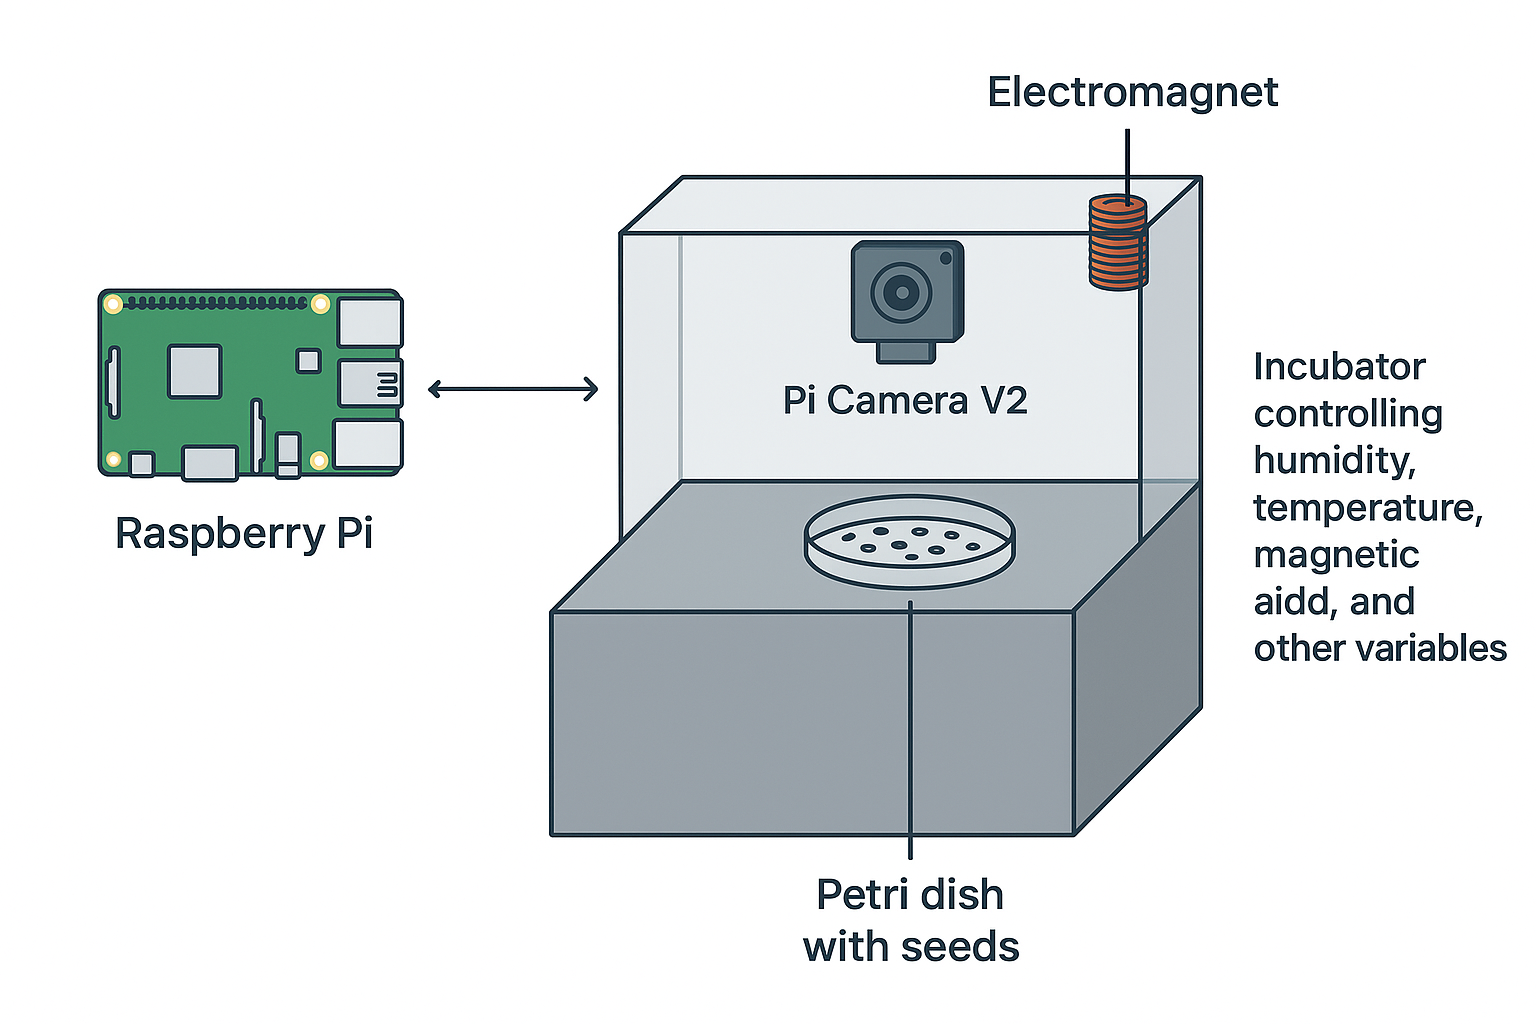
\includegraphics[width=0.9\linewidth]{Tesis_presentation/Figures/diagram_prototype_germination_ia.png}
                \caption*{\scriptsize Automated monitoring prototype schematic.}
            \end{figure}
        \end{column}
        
        \begin{column}{0.48\textwidth}
            \vspace{0.3cm}
            \textbf{Grupo de Investigación - UdC}
            \begin{itemize}
                \item \textbf{Grupo:} Investigación en Campos Electromagnéticos, Medioambiente y Salud Pública.
                \item \textbf{Líder:} Javier Ignacio Torres Osorio.
                \item \textbf{Trayectoria:} +10 years of experience in \textbf{(TMS)}.
                \item \textbf{Resources:} Use of 6 calibrated incubators for seed stimulation.
                \item Study of \textit{Solanum lycopersicum} (Tomato).
            \end{itemize}
        \end{column} 
    \end{columns}
\end{frame}

\begin{frame}{Prototype and Annotation Scheme}     
    \vspace{-0.2cm}
    \begin{columns}[T]
        \begin{column}{0.48\textwidth}
            \vspace{0.6cm}
            \centering
            \begin{figure}
                \centering                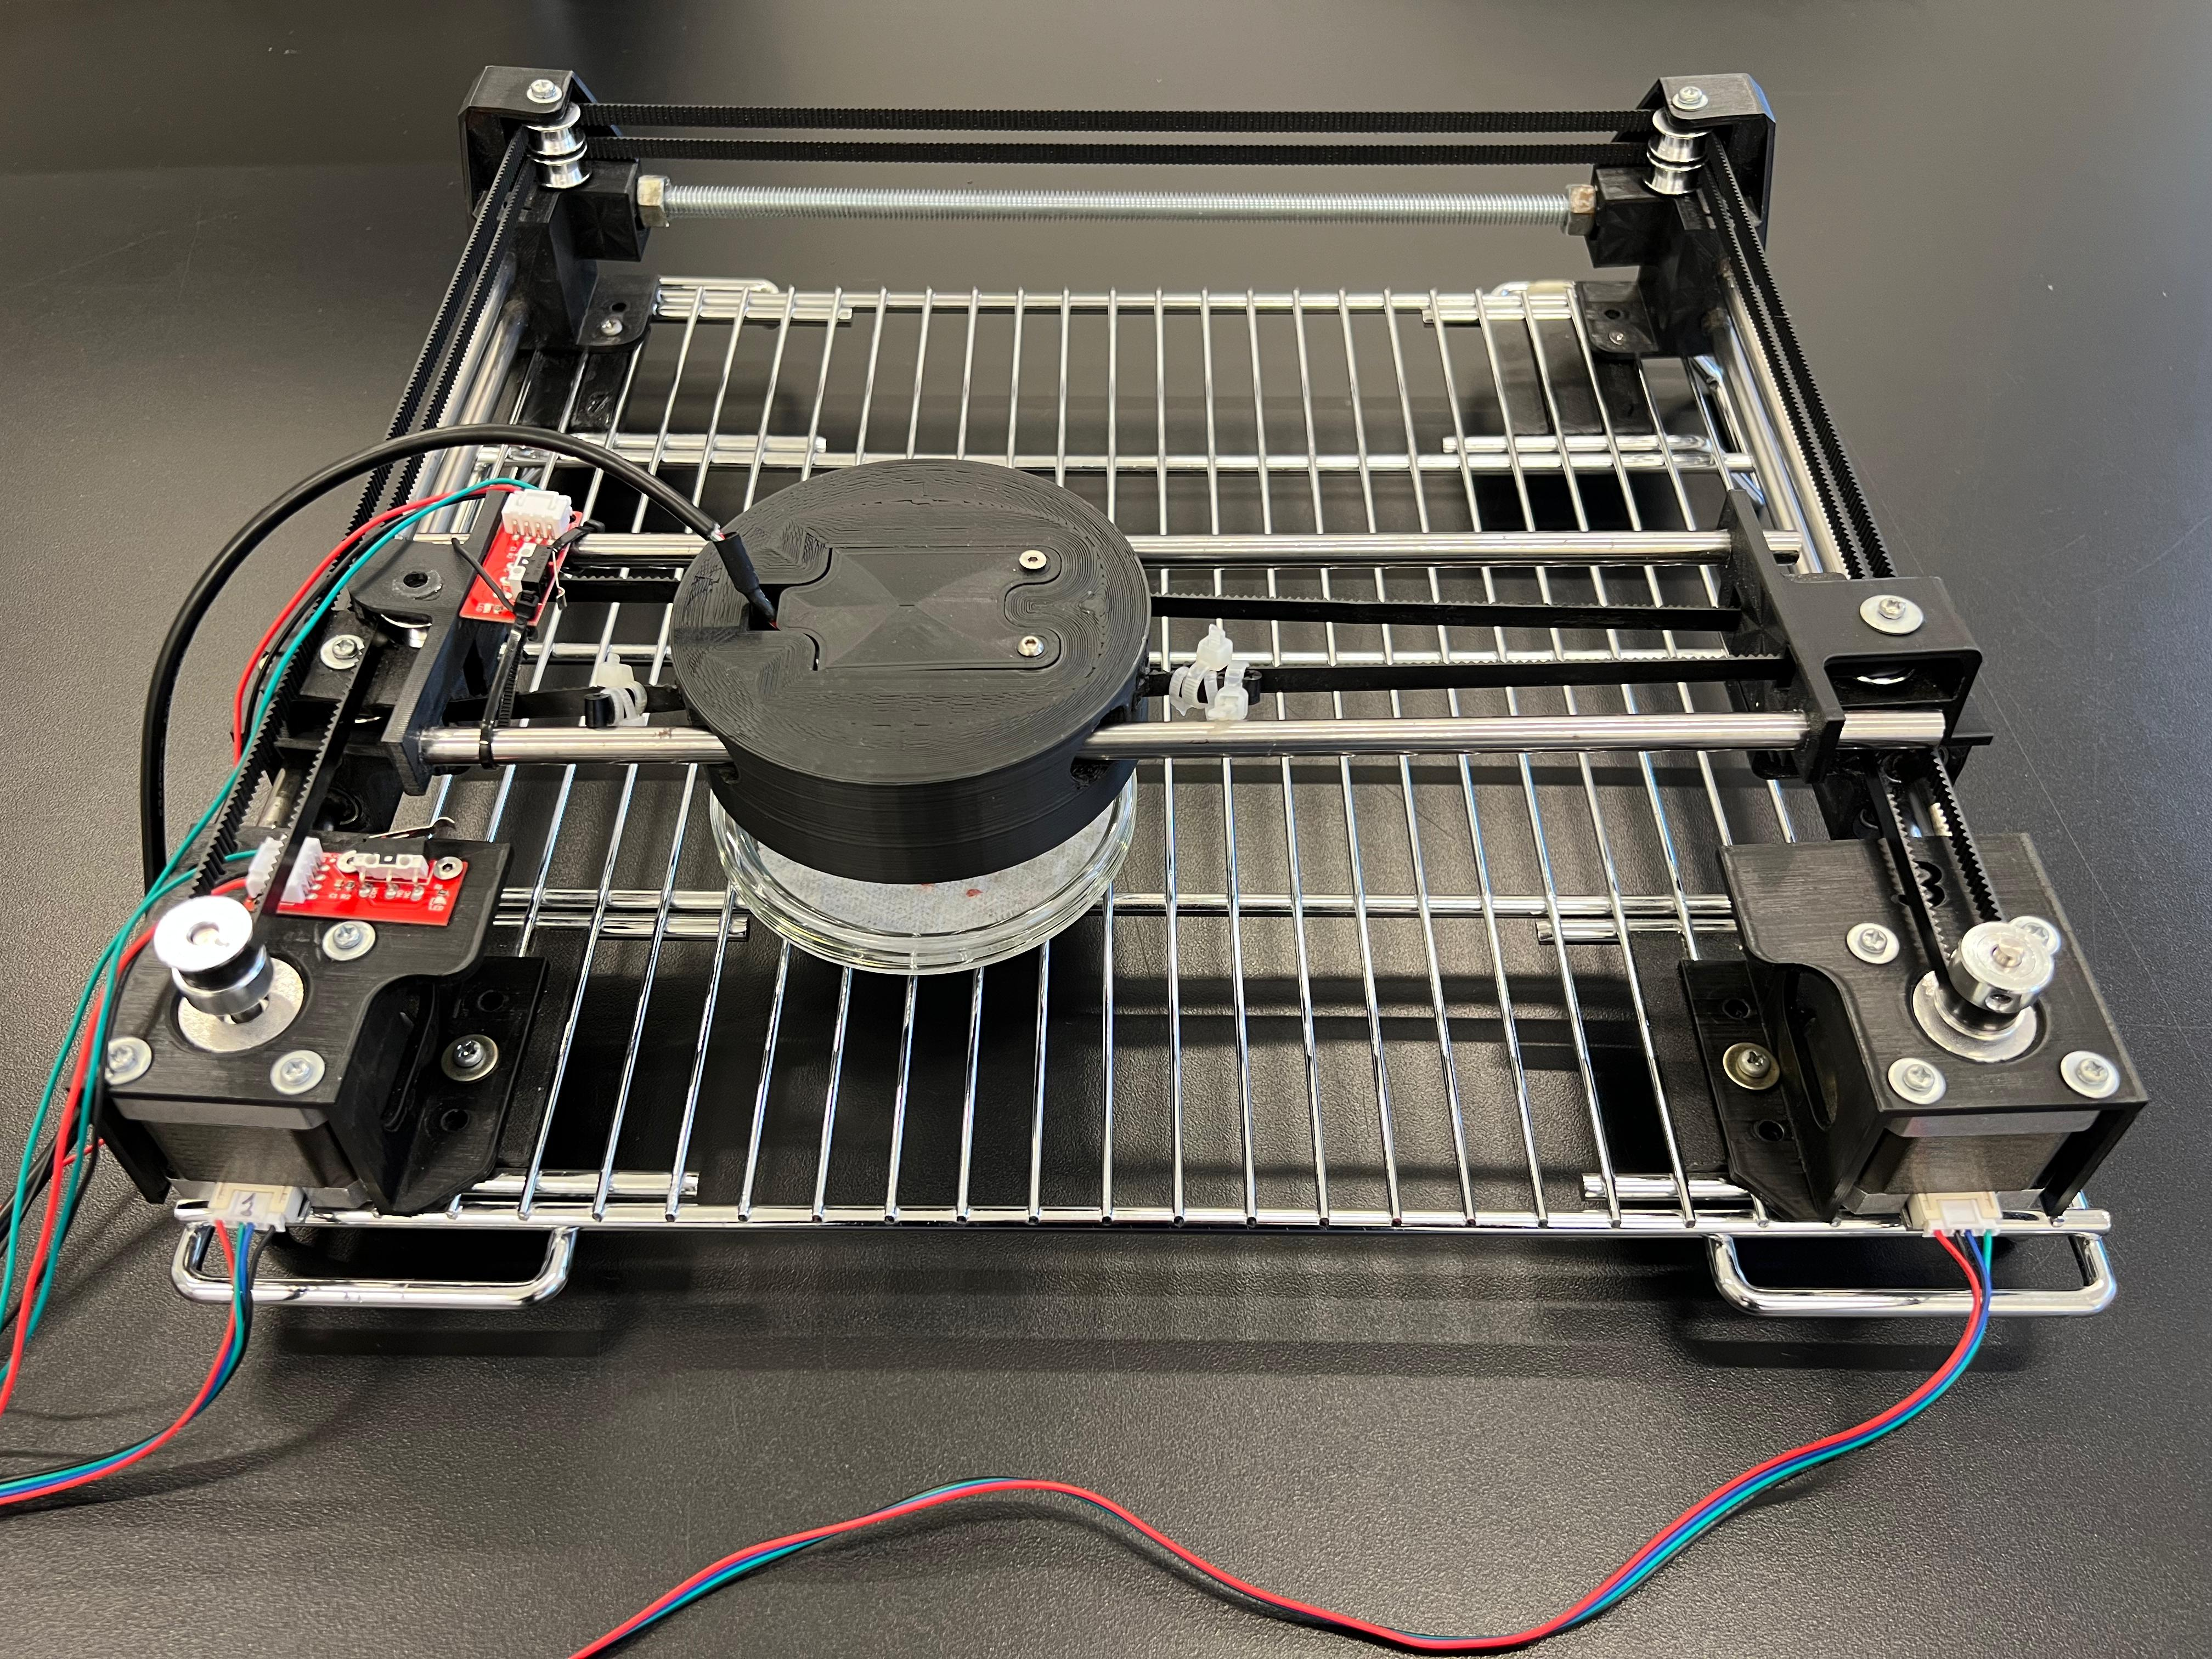
\includegraphics[width=0.8\linewidth]{Tesis_presentation/Figures/prototipo_1.jpeg}
                \caption{\textbf{Prototype:} Automated acquisition system for \textit{in vitro} germination analysis in \textit{Solanum lycopersicum}.}
            \end{figure}
        \end{column}
        
        \begin{column}{0.48\textwidth}
            \begin{exampleblock}{Semantic Annotation}
                \begin{itemize}
                    \item \textbf{Background:} Non-seed pixels
                    \item \textbf{\textcolor{red}{Germinated}:} Radicle $\geq$ 1 mm
                    \item \textbf{\textcolor{brown!60!white}{Non-Germinated}:} Radicle $<$ 1 mm
                \end{itemize}
            \end{exampleblock}
            \vspace{-0.3cm}
            \begin{figure}
                \centering
                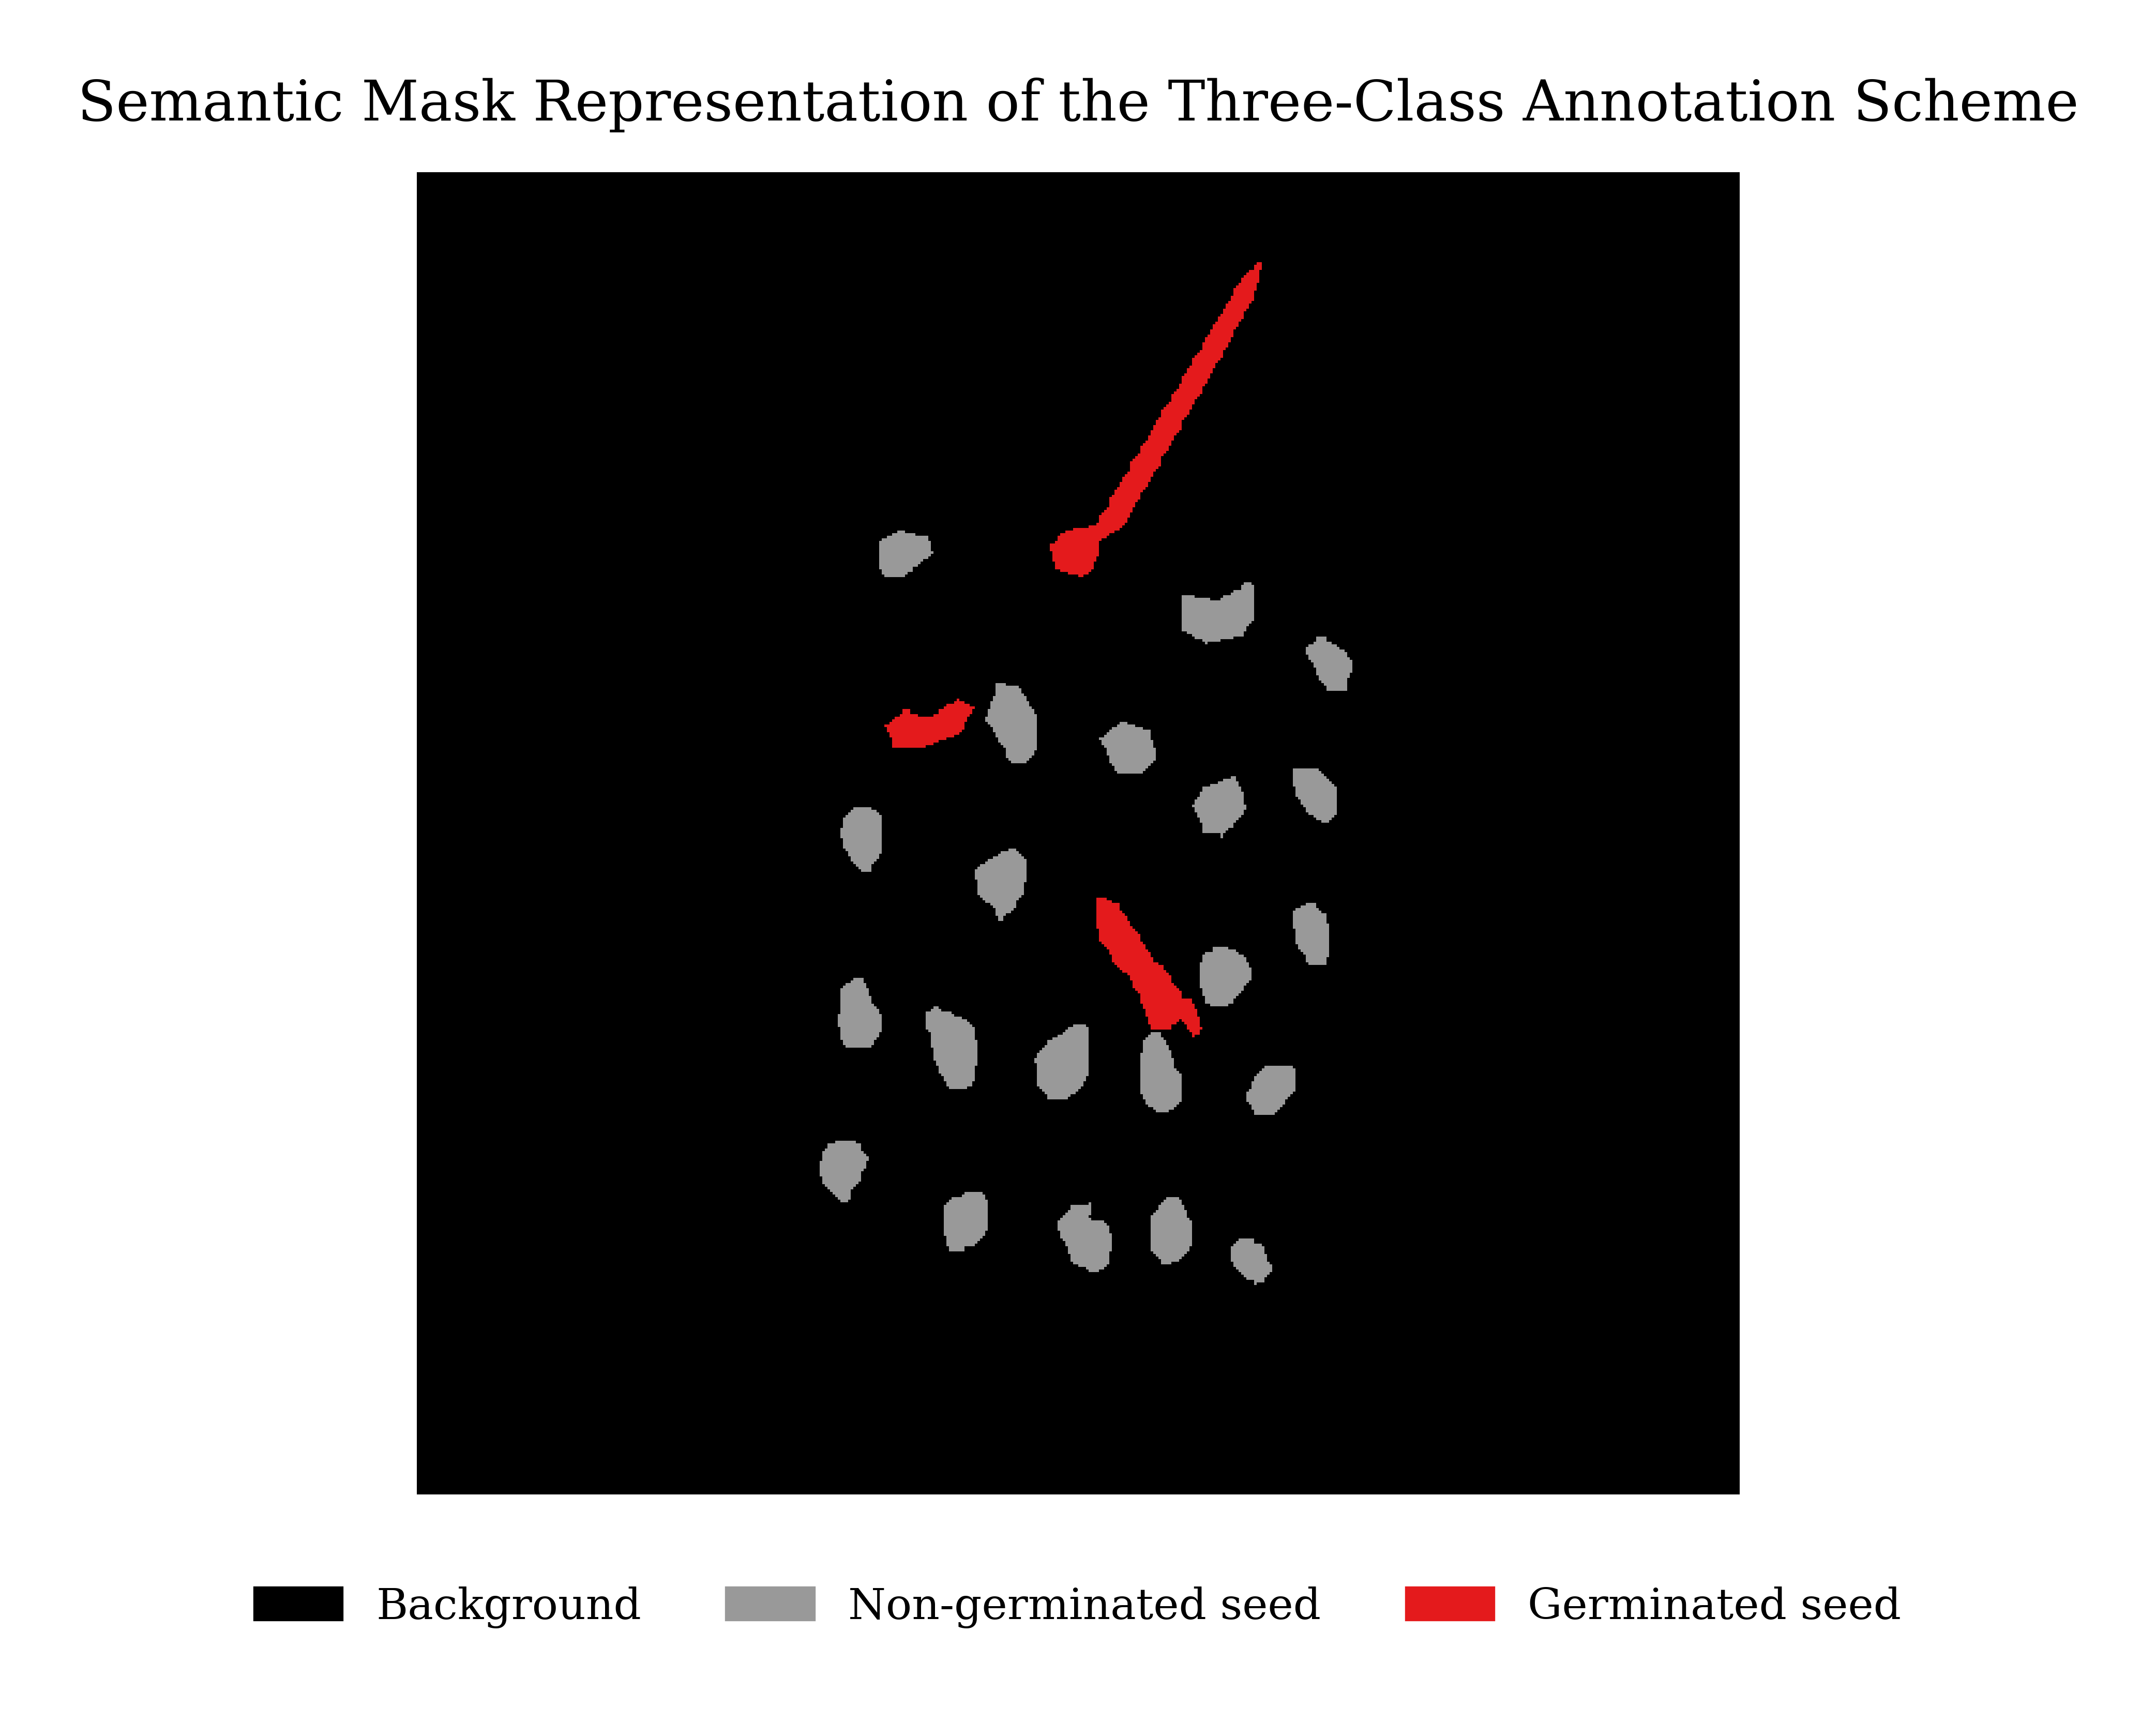
\includegraphics[width=0.8\linewidth]{Tesis_presentation/Figures/semantic_mask_three_classes_paper.png}
            \end{figure}
        \end{column}
    \end{columns}
\end{frame}

\begin{frame}{Dataset Challenges}
    \begin{columns}[T]
        \begin{column}{0.48\textwidth}
            \begin{alertblock}{Intrinsic Technical Challenges}
                \footnotesize
                \begin{itemize}
                    \item \textbf{Low Visual Contrast:} High intensity similarity between the seed coat and background, especially in early stages.
                    \item \textbf{Photometric Instability:} Lighting drifts and reflections caused by the incubator's LED PWM and internal environment.
                \end{itemize}
            \end{alertblock}
        \end{column}
        
        \begin{column}{0.48\textwidth}
            \begin{alertblock}{Morphological Complexity}
                \footnotesize
                \begin{itemize}
                    \item \textbf{Partial Occlusions:} Overlapping seeds and emerging radicles in high-density Petri dishes.
                    \item \textbf{Data Scarcity:} Only 1,578 manually annotated images, necessitating a robust expansion strategy to prevent overfitting.
                \end{itemize}
            \end{alertblock}
        \end{column}
    \end{columns}
    \vspace{0.4cm}
    \centering
    \scriptsize
    \textit{These factors require a strategy that increases sample diversity without compromising the subtle biological features used for germination detection.}
\end{frame}

\begin{frame}{Methodological Pipeline Overview}
    \begin{columns}[T, onlytextwidth]
        \begin{column}{0.4\textwidth}
            \begin{figure}
                \centering
                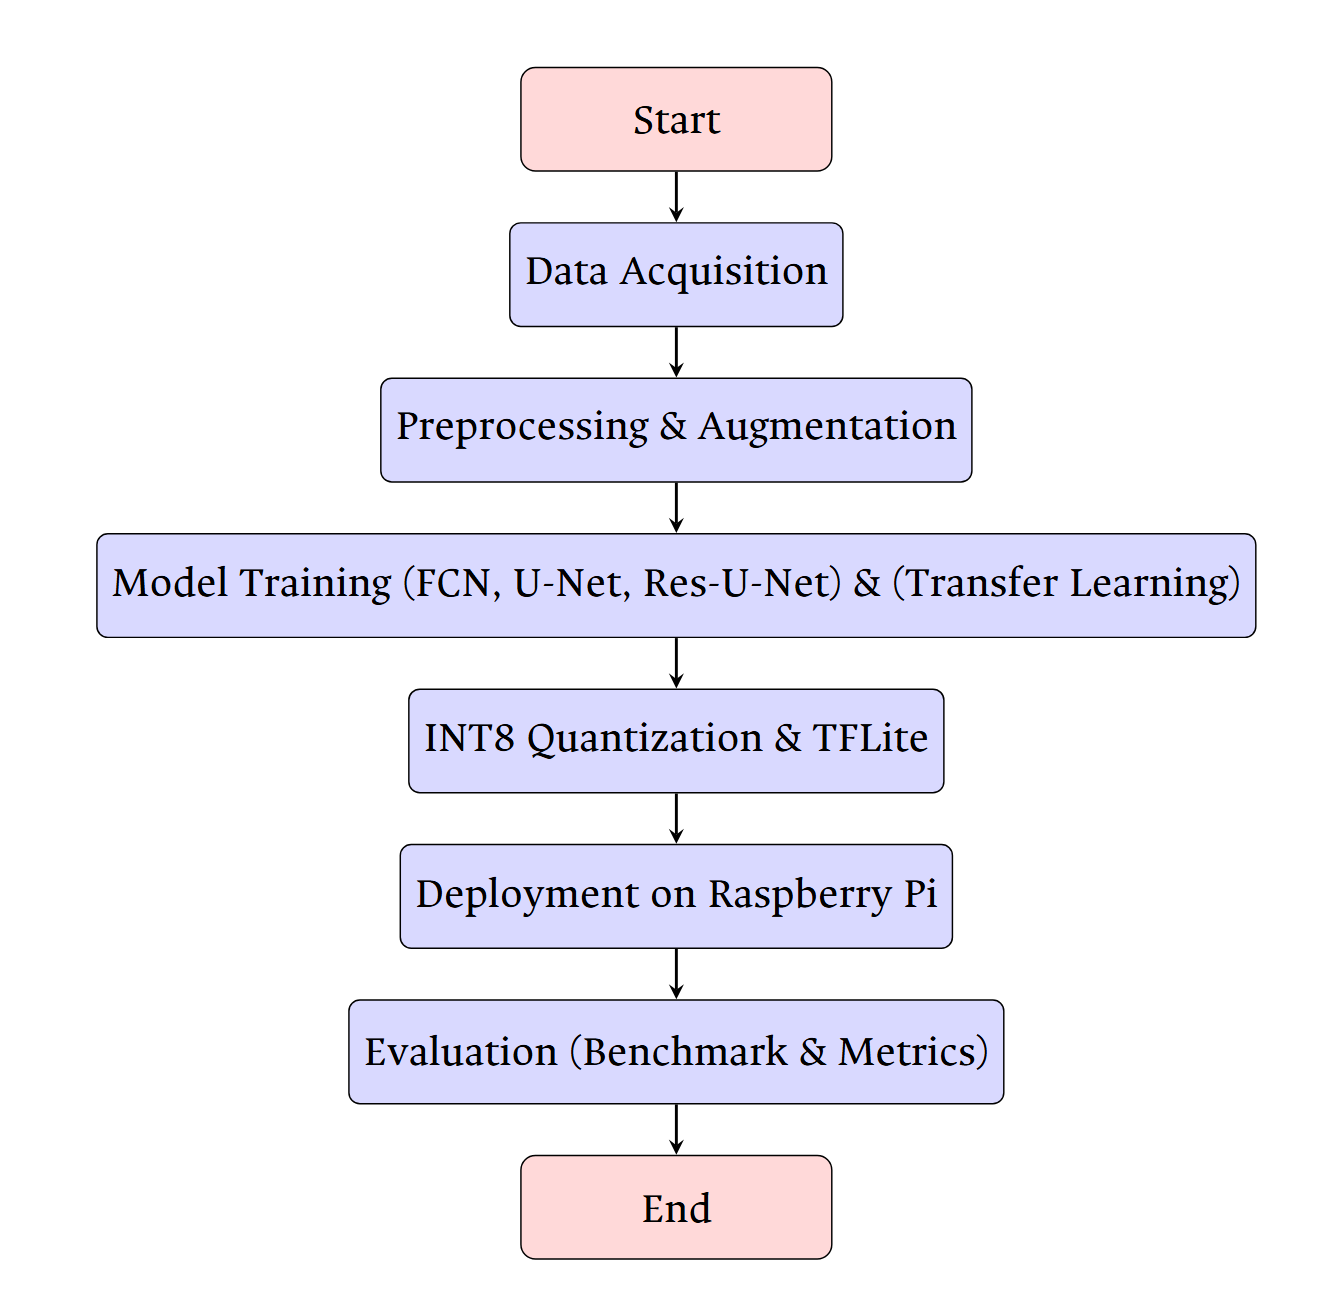
\includegraphics[width=\linewidth]{Tesis_presentation/Figures/pipeline_proposed.png}
            \end{figure}
        \end{column}

        \begin{column}{0.48\textwidth}
            \begin{block}{Four-Stage Strategy}
                \scriptsize
                \begin{enumerate}
                    \item \textbf{Data: Simple Augmentation \textcolor{blue}{(Obj1, Obj2)}} 
                    \\ $\rightarrow$ \textit{Benefit:} Mitigates lighting/contrast issues while preserving \textbf{biological morphology} (prevents GAN hallucinations).
                
                    \item \textbf{Training: Transfer Learning + Segmentation \textcolor{blue}{(Obj1, Obj2)}}
                    \\ $\rightarrow$ \textit{Benefit:} Solves data scarcity and ensures \textbf{pixel-level precision}.
                
                    \item \textbf{Optimization: INT8 Quantization \textcolor{blue}{(Obj3)}}
                    \\ $\rightarrow$ \textit{Benefit:} \textbf{$4\times$ size reduction} and CPU acceleration for efficient real-time execution.
                
                    \item \textbf{Deployment: Raspberry Pi 3B+ \textcolor{blue}{(Obj3)}}
                    \\ $\rightarrow$ \textit{Benefit:} High \textbf{cost-efficiency} for embedded \textit{in vitro} phenotyping without GPU dependency.
                \end{enumerate}
            \end{block}
        \end{column}
    \end{columns}
\end{frame}



\begin{frame}{High-Fidelity Augmentation Strategy}
    \begin{columns}[T]
        \begin{column}{0.43\textwidth}
            \vspace{1.4cm}
            \begin{exampleblock}{Addressing Challenges}
                \scriptsize
                \begin{itemize}
                    \item \textbf{Exposure ($\pm 14\%$) \& Noise:} Mitigates \textbf{Low Contrast} and \textbf{Photometric Instability} by simulating sensor drifts.
                    \item \textbf{Rotation \& Zoom:} Provides \textbf{Spatial Invariance} for seeds in any orientation or scale.
                    \item \textbf{Increase in samples:} Effectively ($1,578 \rightarrow 2,807$ total samples).
                \end{itemize}
            \end{exampleblock}
        \end{column}

        \begin{column}{0.53\textwidth}
            \vspace{-0.5cm}
            \begin{figure}
                \centering
                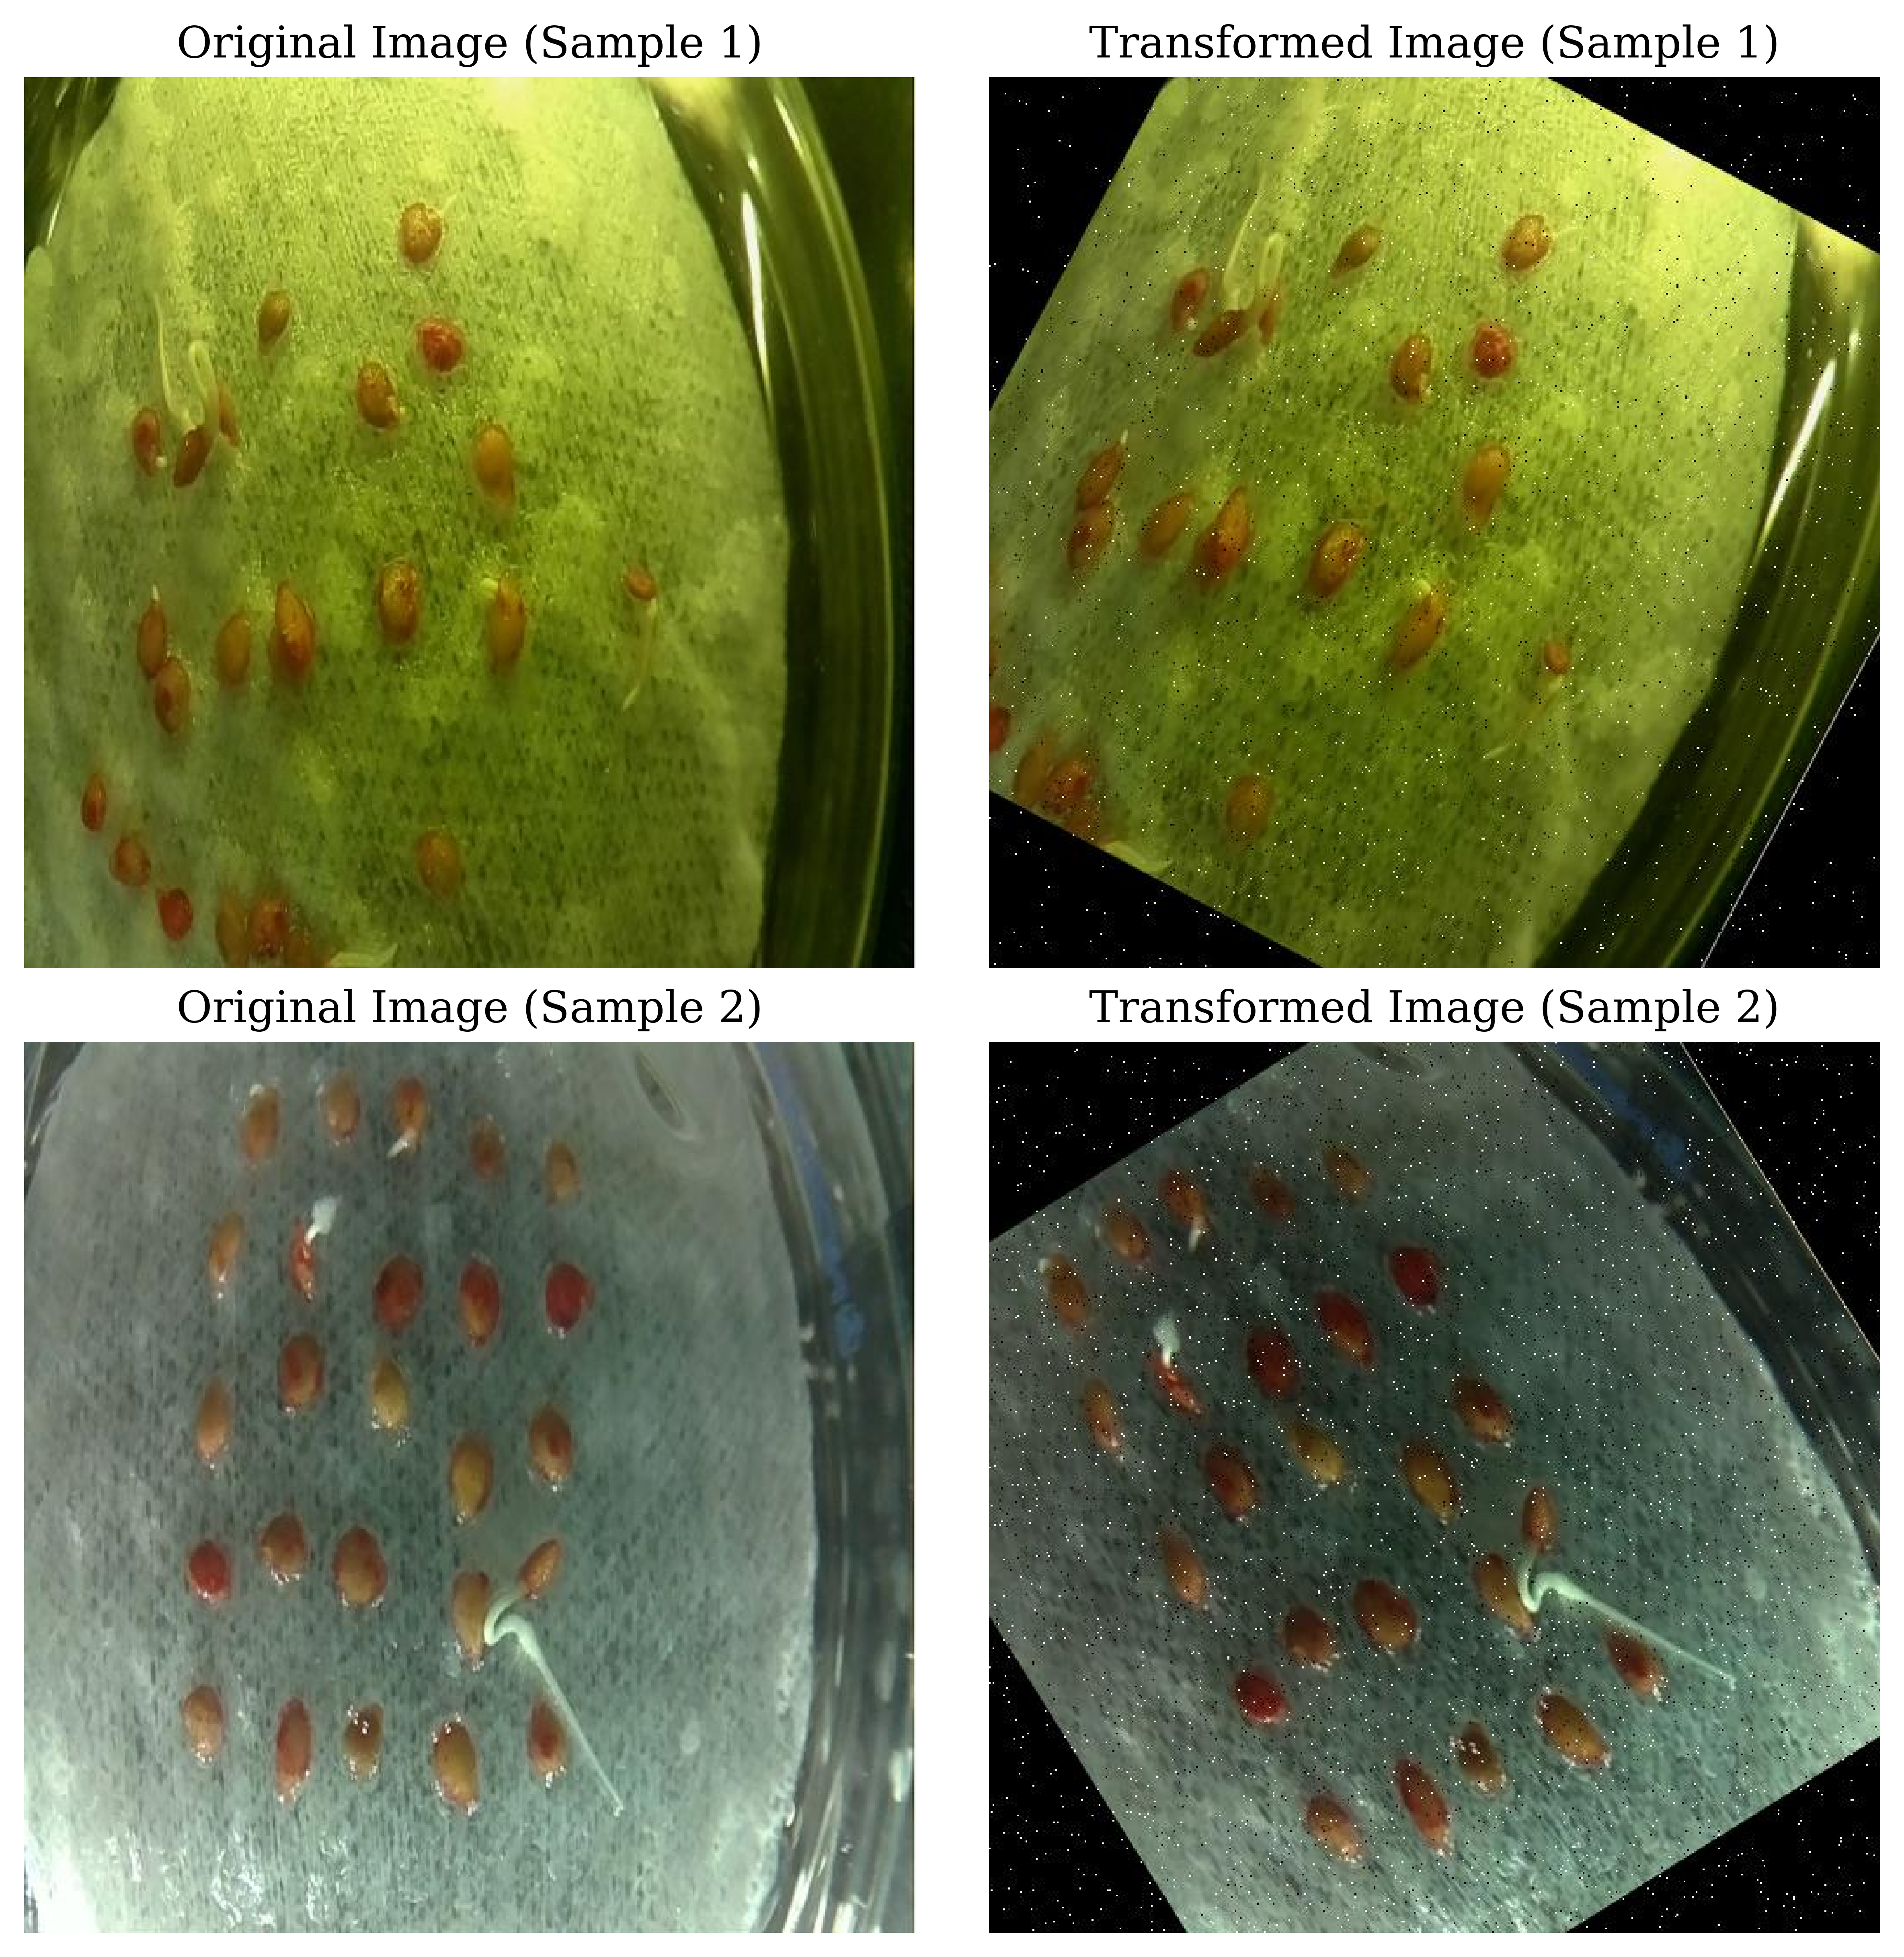
\includegraphics[width=0.85\linewidth]{Tesis_presentation/Figures/mosaico_transformations_paper.png}
            \end{figure}
        \end{column}
    \end{columns}
\end{frame}

\begin{frame}{Semantic Segmentation fundaments}

\textbf{Objective:} Learn a pixel-wise mapping
\[
f_{\boldsymbol{\theta}}:\;\mathbb{R}^{H \times W \times 3}
\;\rightarrow\;
[0,1]^{H \times W \times C}
\]

\vspace{0.3cm}

\begin{columns}
\column{0.5\textwidth}
\textbf{Dataset Definition:}
\[
\mathcal{D} = \{(\mathbf{X}_i,\mathbf{Y}_i)\}_{i=1}^{n}
\]

\begin{itemize}
\item $\mathbf{X}_i \in \mathbb{R}^{H \times W \times 3}$: RGB image
\item $\mathbf{Y}_i \in \{0,1\}^{H \times W \times C}$: semantic label map
\item $C$: number of semantic classes
\end{itemize}

\column{0.5\textwidth}
\textbf{optimization problem:}
\[
\boldsymbol{\theta}^* =
\arg\min_{\boldsymbol{\theta}}
\frac{1}{n}\sum_{i=1}^{n}
\mathcal{L}\big(\mathbf{Y}_i, f_{\boldsymbol{\theta}}(\mathbf{X}_i)\big)
\]

% \textbf{Dice-based optimization problem:}
%     $$
% 	 \{\mathbf{W}_l\}^L_{l=1} = \arg\min_{\mathbf{W}_l}
% 		 \mathbb{E} \Big\{ -2 \frac{\mathbf{1}^\top(\mathbf{M}_n \odot \mathbf{\hat{M}}_n)\mathbf{1} + \epsilon}{\mathbf{1}^\top \mathbf{M}_n\mathbf{1} + \mathbf{1}^\top\mathbf{\hat{M}}_n\mathbf{1} + \epsilon} 
%  \ : \ \ \forall \ n \in \{1,2,\dots,N \Big\} ,\label{eq:opt}
%     $$
    
% \hfill \textbf{\footnotesize{$\odot$ stands for the element-wise product, and  $\epsilon {=} 1$ avoids numerical instability.}}

\textbf{Output:}
\[
\mathbf{P}_i = f_{\boldsymbol{\theta}}(\mathbf{X}_i)
\in [0,1]^{H \times W \times C}
\]
\end{columns}

\vspace{0.25cm}
\small
\textit{Enables dense pixel-level prediction required for morphological trait extraction during seed germination.}

\footnotetext[1]{\scriptsize Semantic segmentation with CNNs \cite{Minaee2021, long2015fully, luo2024semseg}}

\end{frame}


\begin{frame}{Tested architectures}
\begin{figure}
    \centering
    \begin{subfigure}[b]{0.5\textwidth}
        \centering
        \includegraphics[width=\textwidth]{Tesis_presentation/Figures/fcn_architecture.pdf}
    \end{subfigure}
    \hfill
    \begin{subfigure}[b]{0.48\textwidth}
        \centering
        \includegraphics[width=\textwidth]{Tesis_presentation/Figures/unet_architecture.pdf}
    \end{subfigure}
    
    \vspace{-5em}
    \begin{subfigure}[b]{0.48\textwidth}
        \centering
        \includegraphics[width=\textwidth]{Tesis_presentation/Figures/resunet_architecture_readable.pdf}
    \end{subfigure}
    \hfill
    \begin{subfigure}[b]{0.48\textwidth}
        \centering
        \vspace{2cm}
        \begin{align*}
        f_{\text{FCN}}(\mathbf{X}) &= (\ \phi_L \circ \phi_{L-1} \circ \cdots \circ \phi_1 )(\mathbf{X}) \\[1.5em]
        f_{\text{UNet}}(\mathbf{X}) &= \mathcal{D}\big(\mathcal{E}(\mathbf{X}), \mathcal{S}(\mathbf{X})\big) \\[1.5em]
        f_{\text{ResUNet}}(\mathbf{X}) &= \mathcal{D}_{\text{res}}\big(\mathcal{E}_{\text{res}}(\mathbf{X}), \mathcal{S}_{\text{res}}(\mathbf{X})\big)
        \end{align*}
    \end{subfigure}
\end{figure}
\end{frame}

\begin{frame}{Transfer learning procedure}
    \begin{figure}[!ht]
        \centering        \includegraphics[width=0.65\linewidth, trim={0 0 0 100pt}, clip]{Tesis_presentation/Figures/transfer_learning_architectures.pdf}
    \end{figure}
\end{frame}

\begin{frame}{Evaluation Metrics: Segmentation \& Geometry}
    \begin{columns}[T, onlytextwidth]
        \column{0.48\textwidth}
        \begin{block}{Overlap-Based Metrics}
            \scriptsize
            \[ \mathrm{Dice}(P,T) = \frac{2|P \cap T| + \varepsilon}{|P| + |T| + \varepsilon} \]
            \[ \mathrm{IoU}(P,T) = \frac{|P \cap T| + \varepsilon}{|P \cup T| + \varepsilon} \]
            \textit{Evaluates spatial overlap between predicted and ground-truth masks.}
            \[ \mathrm{mAP} = \frac{1}{C} \sum_{c=1}^{C} \left[ \frac{1}{K} \sum_{k=1}^{K} \mathbf{1}(\mathrm{IoU}_c > \tau_k) \right] \]
            \textbf{mAP@50-95:} Decisive for sub-pixel boundary precision in phenotyping.
        \end{block}

        \column{0.48\textwidth}
        \begin{block}{Classification}
            \scriptsize
            \[
            \mathrm{Sens.} = \frac{\mathrm{TP}}{\mathrm{TP} + \mathrm{FN} + \varepsilon}
            \qquad
            \mathrm{Spec.} = \frac{\mathrm{TN}}{\mathrm{TN} + \mathrm{FP} + \varepsilon}
            \]
            \[
            \mathrm{Prec.} = \frac{\mathrm{TP}}{\mathrm{TP} + \mathrm{FP} + \varepsilon}
            \]
        \end{block}

        \begin{exampleblock}{Key Training Parameters}
            \scriptsize
            \begin{itemize}
                \item \textbf{Loss:} Dice-based Loss.
                \item \textbf{Optimizer:} Adam ($LR=1\times10^{-4}$).
                \item \textbf{Epochs:} 60.
                \item \textbf{Platform:} \href{https://www.kaggle.com/}{Kaggle.}
                \item \textbf{Hardware:} 2$\times$ NVIDIA V100 GPUs.
            \end{itemize}
        \end{exampleblock}
    \end{columns}
\end{frame}

\begin{frame}{Examples of segmentation}
    \begin{figure}
        \centering
        \includegraphics[width=0.75\linewidth]{Tesis_presentation/Figures/segmentation_example.png}
    \end{figure}
\end{frame}

\begin{frame}{Effect of Transfer Learning and Generalization}
    \begin{columns}[T, onlytextwidth]
        \begin{column}{0.65\textwidth}
            \begin{figure}
                \centering
                \includegraphics[width=\linewidth]{Tesis_presentation/Figures/size_vs_metrics_comparison.pdf}
            \end{figure}
        \end{column}

        \begin{column}{0.33\textwidth}
            \begin{exampleblock}{Generalization Strategies}
                \small Robustness achieved through two distinct paths:
            \end{exampleblock}

            \begin{itemize}
                \scriptsize
                \item \textbf{Non-linear overlap:} Germinated vs. non-germinated seeds are visually similar.
                \item \textbf{Simplicity:} FCN (scratch) generalizes better than U-Net (scratch) by constraining complexity.
                \item \textbf{External Knowledge (TL):} Pre-trained MobileNetV2 provides the best results. +3.96 \% over VGG16, +4.51 \% (scratch). 
            \end{itemize}
        \end{column}
    \end{columns}
\end{frame}

\begin{frame}{Segmentation results}
        \begin{table}[H]
    \centering
    \label{tab:compare_best}
    \small
    \setlength{\tabcolsep}{4pt}
    \begin{tabular}{l|c|c|c|c|c|c|c}
    \hline
    \textbf{Model} & \textbf{Var.} & \textbf{Dice} & \textbf{Jaccard} & \textbf{Sens.} & \textbf{Spec.} & \textbf{mAP@50} & \textbf{mAP@50-95} \\
    \hline
    UNetImageNetMobV2 & 3c & 0.84 & 0.79 & 0.80 & 0.97 & 0.87 & 0.70 \\
    ResUNetImageNetMobV2 & 3c & 0.82 & 0.77 & 0.80 & 0.98 & 0.87 & 0.69 \\
    ImageNetMobV2 & 3c & 0.82 & 0.77 & 0.77 & 0.96 & 0.86 & 0.66 \\
    FCN & 3c & 0.82 & 0.77 & 0.77 & 0.96 & 0.84 & 0.66 \\
    \hline
    \end{tabular}
    \end{table}


    \begin{exampleblock}{Transfer Learning (TL) Impact}
        \scriptsize
        \begin{itemize}
            \item \textbf{Scratch Collapse:} Models without priors (TL) fail to learn the complex decision boundary.
            \item \textbf{Regularization:} TL acts as a data amplifier for small datasets, +6.2\% Dice and +10.7\% mAP@50 vs scratch-trained models.
            \item \textbf{Geometric accuracy:} UNet-MobV2 and ResUNet-MobV2 provides a good balance in geometric accuracy (mAP@50:95).
        \end{itemize}
    \end{exampleblock}

\end{frame}

\begin{frame}{Post-Training INT8 Quantization}
    \begin{columns}[T, onlytextwidth]
        \column{0.48\textwidth}
        \begin{block}{Affine Mapping (FP32 $\to$ INT8)}
            \scriptsize
            \[ r = S(q - Z) \]
            \textbf{Parameters:}
            \[ s = \frac{T_{\max} - T_{\min}}{255} \]
            \[ z = \mathrm{round}\!\left(0 - \frac{T_{\min}}{s}\right) \]
        \end{block}
        \begin{block}{Quantized Inference}
            \tiny
            \[ t_q = \mathrm{clip} \left( \mathrm{round}\!\left(\frac{t}{s}\right) + z,\; 0,\; 255 \right) \]
        \end{block}

        \column{0.48\textwidth}
        \begin{exampleblock}{Implementation in TFLite}
            \scriptsize
            \begin{itemize}
                \item \textbf{Calibration:} Representative dataset to estimate dynamic ranges ($T_{\max}, T_{\min}$).
                \item \textbf{Benefit:} Mandatory for ARM platforms to achieve practical latency.
                \item \textbf{Justification:} Superior maturity for post-training INT8 quantization \cite{kang2022evaluation}, a non-negotiable requirement for mitigating hardware performance bottlenecks.
            \end{itemize}
        \end{exampleblock}
    \end{columns}
\end{frame}

\begin{frame}{Edge Deployment Environment}
    \begin{columns}[c, onlytextwidth]
        \column{0.48\textwidth}
        \begin{alertblock}{Edge Constraints}
            \scriptsize
            \begin{itemize}
                \item Resource-limited ARM CPUs.
                \item Critical memory footprint (RAM).
                \item Need for specialized runtimes (TFLite + XNNPACK).
            \end{itemize}
        \end{alertblock}

        \begin{block}{Raspberry Pi 3B+}
            \scriptsize
            \begin{itemize}
                \item \textbf{CPU:} 1.4GHz Cortex-A53 (4 cores).
                \item \textbf{RAM:} 1GB LPDDR2 SDRAM.
                \item \textbf{OS:} Manjaro ARM.
            \end{itemize}
        \end{block}

        \column{0.48\textwidth}
        \centering
        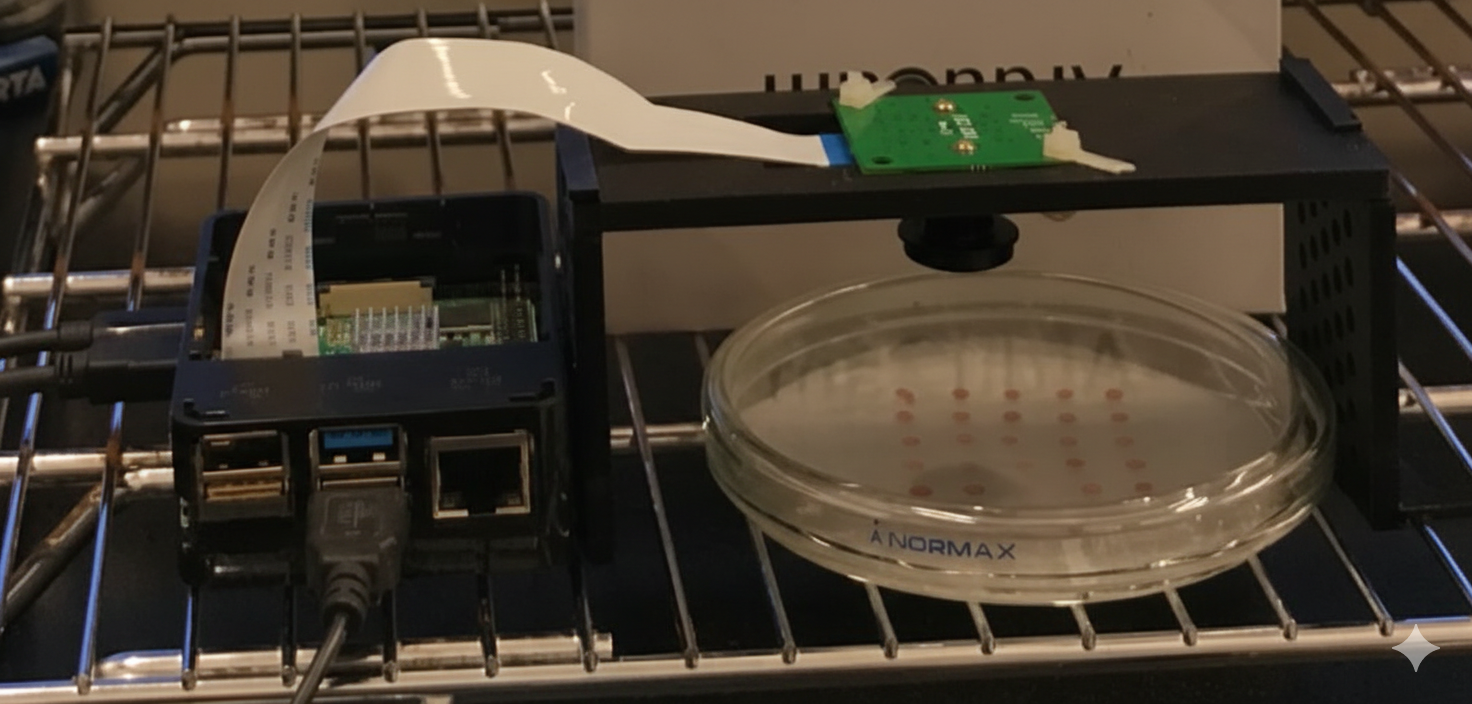
\includegraphics[width=\linewidth]{Tesis_presentation/Figures/pi_setup.png} % Ajustar ruta
        \vspace{0.5em}
        \caption{\tiny \textbf{Target Hardware:} Balanced platform for periodic germination monitoring.}
    \end{columns}
\end{frame}

\begin{frame}{Embedded Performance and Trade-offs}
    \begin{columns}[T, onlytextwidth]
        \column{0.48\textwidth}
        \begin{block}{Model Selection (3-Class)}
            \centering
            \tiny
            \begin{tabular}{l c c c c}
                \toprule
                \textbf{Model} & \textbf{Rnk} & \textbf{MB} & \textbf{Dice} & \textbf{mAP@50:95} \\
                \midrule
                FCN (scratch) & 1.3 & 4.6 & 0.82 & 0.66 \\
                \textbf{ResUNetMobV2} & \textbf{1.8} & \textbf{14.5} & \textbf{0.84} & \textbf{0.87} \\
                MobV2 Backbone & 3.8 & 21.4 & 0.84 & 0.70 \\
                UNetMobV2 & 4.2 & 24.8 & 0.84 & 0.70 \\
                \bottomrule
            \end{tabular}
        \end{block}
        
        \vspace{-0.5em}
        \begin{itemize}
            \tiny
            \item \textbf{ResUNetMobV2:} Best balance for phenotyping.
            \item VGG16 models are too heavy for edge use.
        \end{itemize}

        \column{0.48\textwidth}
        \begin{exampleblock}{TFLite Benchmark (RPi 3)}
            \centering
            \tiny
            \begin{tabular}{l l c c c c}
                \toprule
                \textbf{Model} & \textbf{Type} & \textbf{MB} & \textbf{FPS} & \textbf{Dice} & \textbf{mAP@50:95} \\
                \midrule
                \textbf{ResUNetMobV2} & FP32 & 14.4 & 0.3 & 0.84 & 0.71 \\
                \textbf{ResUNetMobV2} & \textbf{INT8} & \textbf{4.1} & \textbf{0.5} & \textbf{0.84} & \textbf{0.68} \\
                \midrule
                FCN (scratch) & FP32 & 4.6 & 0.04 & 0.81 & 0.64 \\
                FCN (scratch) & \textbf{INT8} & \textbf{1.2} & 0.4 & \textbf{0.75} & \textbf{0.58} \\
                \bottomrule
            \end{tabular}
        \end{exampleblock}
        
        \vspace{-0.5em}
        \begin{itemize}
            \tiny
            \item \textbf{Quantization:} $3.5\times$ size reduction.
            \item \textbf{FCN Fragility:} Dice drops $\approx 6$ pts in INT8.
        \end{itemize}
    \end{columns}
\end{frame}

\begin{frame}{Quantitative strategy deployed}
    \begin{columns}[c]
        \column{0.45\textwidth}
        \begin{alertblock}{FCN Failure}
            \small Simplicity leads to high quantization sensitivity; lacks skip connections.
        \end{alertblock}
        
        \vspace{1em}
        
        \begin{exampleblock}{ResUNet Robustness}
            \small Redundancy in MobileNetV2 filters buffers numerical errors.
        \end{exampleblock}
        
        \column{0.55\textwidth}
        \begin{figure}
            \centering            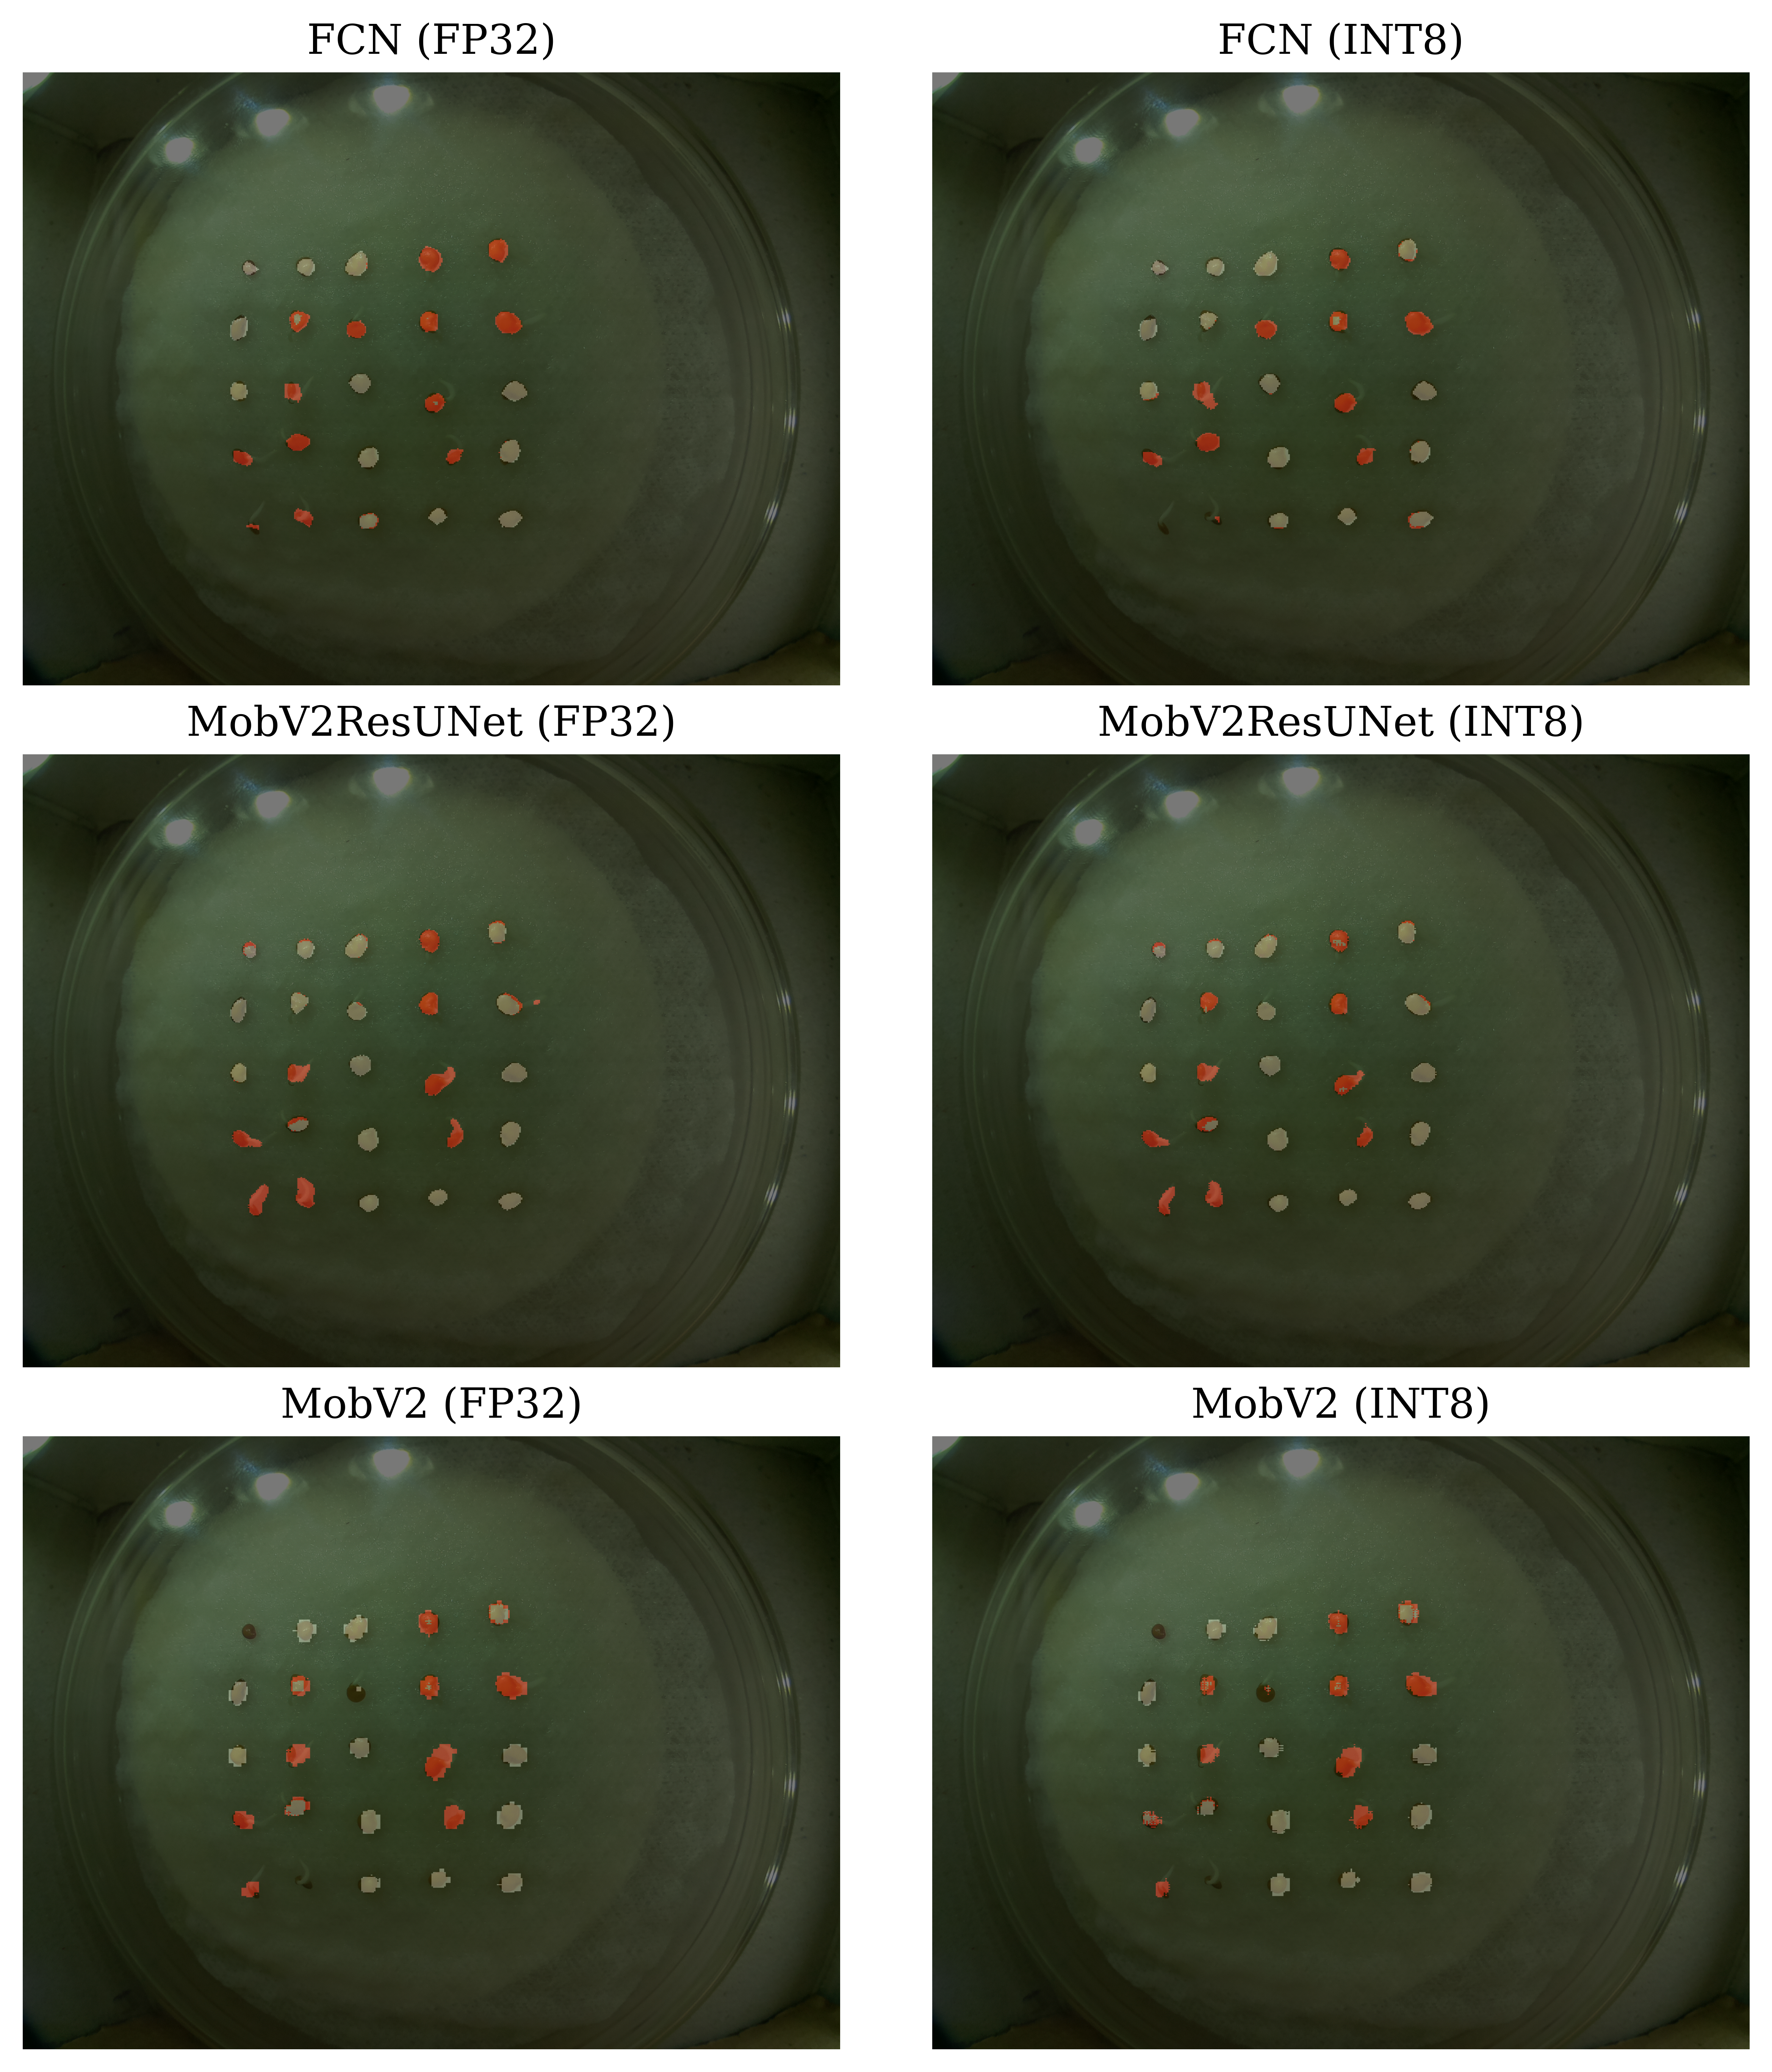
\includegraphics[width=0.7\linewidth]{Tesis_presentation/Figures/mosaico_predicciones_paper.png}
        \end{figure}
    \end{columns}
\end{frame}

\section{Conclusions and  Future Work}

\begin{frame}{Conclusions}
    \begin{itemize}
        \item \textbf{Objective 1: CNN Architecture Evaluation}
                \small
                \begin{itemize}
                    \item \textbf{Best Architecture:} ResUNet with MobileNetV2 backbone achieved best balance
                    \item \textbf{Performance:} 0.84 Dice, 0.79 Jaccard, 0.87 mAP@50 in challenging 3-class segmentation
                    \item \textbf{Validation:} Pixel-level segmentation outperforms bounding-box detection for fine morphological analysis
                \end{itemize}
        
        \vspace{0.5em}
        \item \textbf{Objective 2: Transfer Learning \& Data Augmentation}
                \small
                \begin{itemize}
                    \item \textbf{Effective Strategy:} Augmentation mitigated data scarcity (1,578 $\rightarrow$ 2,807 samples)
                    \item \textbf{Performance Gain:} +6.2\% Dice and +10.7\% mAP@50 vs scratch-trained models
                    \item \textbf{Best Backbone:} MobileNetV2 consistently outperformed VGG16 in all metrics
                \end{itemize}
        
        \vspace{0.5em}
        \item \textbf{Objective 3: Edge Deployment via Quantization}
                \small
                \begin{itemize}
                    \item \textbf{Efficiency:} INT8 quantization achieved 3.5$\times$ size reduction, 26\% faster inference
                    \item \textbf{Accuracy Preservation:} Minimal accuracy loss ($<$3\%) post-quantization
                    \item \textbf{Feasibility:} 0.5 FPS on Raspberry Pi 3 enables periodic monitoring
                \end{itemize}
    \end{itemize}
    
    \vspace{1em}
    \centering
    \textbf{Final Solution:} ResUNetImageNetMobV2 INT8 \\
    \small (0.84 Dice, 4.07 MB, 0.5 FPS on Raspberry Pi 3)
    
    \vspace{0.5em}
    \footnotesize \textit{A reproducible, lightweight pipeline for automated seed germination monitoring.}
\end{frame}

\begin{frame}{Future Work}
    \begin{itemize}
        \item \textbf{Objective 1: Morphological Precision}
            \begin{itemize}
                \scriptsize
                \item Evaluation of Vision Transformers adapted for small-object and thin-structure segmentation
            \end{itemize}
        
        \item \textbf{Objective 2: Data Efficiency \& Generalization}
            \begin{itemize}
                \scriptsize
                \item Advanced lightweight backbones (e.g., EfficientNet-Lite, MobilenetV3)
                \item Dataset expansion: intermediate germination states
                \item Domain adaptation across seed species
                
            \end{itemize}
        
        \item \textbf{Objective 3: Edge Deployment Optimization}
            \begin{itemize}
                \scriptsize
                \item Advanced compression: pruning, weight clustering, sparsity
                \item device to deploy: ArduinoUnoQ, Raspberry pi 5
                \item Knowledge distillation from large foundation models to compact student architectures
            \end{itemize}
        
        \item \textbf{Integration \& Application}
            \begin{itemize}
                \scriptsize
                \item Validation in greenhouse/field conditions
                \item Real-time monitoring support
            \end{itemize}
    \end{itemize}
\end{frame}

\begin{frame}{Acknowledgements}
    \centering
    I would like to express my heartfelt appreciation to my parents for their unwavering support and encouragement.
    \vspace{1em}
    I would like to express my gratitude to two esteemed professors, Andrés Marino Álvarez Meza, for providing me with invaluable direction during my research. I would also like to thank the members of the Signal Processing and Recognition Group - SPRG at the Manizales branch of Universidad Nacional de Colombia for their thoughtful suggestions and educational discussion.
    
    \vspace{1em}
    Also, I want to thank to the project: Sistema de visión artificial para el monitoreo y seguimiento de efectos analgésicos y anestésicos administrados vía neuroaxial epidural en población obstétrica durante labores de parto para el fortalecimiento de servicios de salud materna del Hospital Universitario de Caldas - SES HUC (Hermes 57661), funded by Universidad Nacional de Colombia.
\end{frame}

% \begin{frame}{Composite Ranking Metric ($rnk\_mean$)}
%     \begin{exampleblock}{Accuracy-Efficiency Trade-off}
%         \scriptsize
%         Systematic model selection based on the Euclidean distance to the \textbf{ideal operating point} (Size = 0, Metric = 1).
%     \end{exampleblock}
    
%     \begin{columns}[T, onlytextwidth]
%         \column{0.48\textwidth}
%         \begin{block}{1. Normalization (Min-Max)}
%             \tiny
%             \[ v^{\prime}_{m,j} = \frac{v_{m,j} - \min(v_{\cdot,j})}{\max(v_{\cdot,j}) - \min(v_{\cdot,j})} \]
%         \end{block}
%         \begin{block}{2. Distance Calculation}
%             \tiny
%             \[ \text{dist}_{m,i} = \sqrt{ (x'_m - 0)^2 + (y'_{i,m} - 1)^2 } \]
%         \end{block}

%         \column{0.48\textwidth}
%         \begin{block}{3. Final Average Rank}
%             \tiny
%             \[ \mathrm{rnk\_mean}_m = \frac{1}{N} \sum_{i=1}^{N} \mathrm{rank}_{m,i} \]
%         \end{block}
%         \begin{itemize}
%             \tiny
%             \item Penalizes heavy models.
%             \item Rewards precision + compact size.
%         \end{itemize}
%     \end{columns}
% \end{frame}

% % ------------------------------------------------------------------------
\begin{frame}[allowframebreaks]%,noframenumbering]
\frametitle{References}
{\tiny 
\bibliographystyle{apalike}
\bibliography{References}
}

\end{frame}

\begin{frame}{CNN Layer Composition}

\textbf{Neural Network as Function Composition:}
\[
f_{\boldsymbol{\theta}}(\mathbf{x})
=
(f_L \circ f_{L-1} \circ \cdots \circ f_1)(\mathbf{x})
\]

\vspace{0.2cm}

\textbf{Differentiable Layer Formulation:}
\[
\mathbf{z}_\ell =
\phi_\ell(\mathbf{W}_\ell \mathbf{z}_{\ell-1} + \mathbf{b}_\ell)
\]

\small
where $\mathbf{W}_\ell$ and $\mathbf{b}_\ell$ denote learnable parameters and
$\phi_\ell(\cdot)$ a non-linear activation function.

\vspace{0.3cm}

\begin{columns}
\column{0.5\textwidth}
\textbf{Convolutional Operation:}
\[
[\mathbf{X} * \mathbf{K}](i,j)
=
\sum_{u}\sum_{v}
\mathbf{K}_{u,v}\,
\mathbf{X}_{i+u,j+v}
\]

\small
Ensures translation equivariance and parameter efficiency.

\column{0.5\textwidth}
\textbf{Key CNN Properties:}
\begin{itemize}
\item Local connectivity
\item Weight sharing
\item Spatial hierarchy
\item Reduced parameter count
\end{itemize}
\end{columns}

\vspace{0.2cm}
\footnotetext[1]{\scriptsize CNNs replace fully connected layers for image-based learning}

\end{frame}

\end{document}